\documentclass[aps,prd,onecolumn,notitlepage,10pt,amsmath,amssymb,amsfonts,nofootinbib]{revtex4-2}

%==============================================================================
% PACKAGES & MACROS
%==============================================================================
\usepackage{bm}
\usepackage{mathtools}
\usepackage{amsthm}
\usepackage{graphicx}
\usepackage{booktabs}
\usepackage{xcolor}
\usepackage{hyperref}
\hypersetup{colorlinks=true,linkcolor=blue!60!black,citecolor=blue!60!black,urlcolor=blue!60!black}

\newtheorem{theorem}{Theorem}
\newtheorem{proposition}{Proposition}
\newtheorem{corollary}{Corollary}
\newtheorem{conjecture}{Conjecture}
\newtheorem{lemma}{Lemma}
\theoremstyle{definition}
\newtheorem{definition}{Definition}
\newtheorem{assumption}{Assumption}
\theoremstyle{remark}
\newtheorem{remark}{Remark}

\newcommand{\Hil}{\mathcal{H}}
\newcommand{\Hs}{\widehat{H}_S}
\newcommand{\Nop}{\widehat{N}}
\newcommand{\Cop}{\widehat{C}}
\newcommand{\Pt}{\widehat{P}_t}
\newcommand{\R}{\mathbb{R}}
\newcommand{\Z}{\mathbb{Z}}
\newcommand{\N}{\mathbb{N}}
\newcommand{\C}{\mathbb{C}}
\newcommand{\Tr}{\operatorname{Tr}}
\newcommand{\Spec}{\operatorname{Spec}}
\newcommand{\pket}[1]{|#1)}
\newcommand{\pbra}[1]{(#1|}

\begin{document}

\title{The Hilbert-Space Quadrature Conjecture:\\
Time as the Wave-Function-Generated Quadrature of Circular Phase}

\author{Steven Michael Allen Owens}
\affiliation{Independent Researcher}

\date{October 18, 2026 (revised version)}

\begin{abstract}
We develop a geometric and operational reading of relational quantum time, which we call the \emph{Hilbert-space quadrature conjecture}: physical time is not an external parameter but is generated by the universal wave function through the quadratic (Born) map acting on the circular $U(1)$ phase structure of a clock sector. Technically the framework rests on the Page--Wootters conditional-probability construction with shift-covariant clock POVMs, as developed in Refs.~\cite{SmithAhmadi2019,Hohn2021,LoveridgeMiyadera2019}; our contributions are interpretive and clarifying rather than a new dynamics. (i)~Using the Zak (Bloch--Floquet) transform we make precise how universal-cover clocks ($\R$) relate to cyclic clocks ($S^1$): exact constraint solutions for arbitrary system spectra live in twisted circle sectors, and a cyclic clock read without its winding number preserves coherence only between levels whose energy difference is an integer multiple of the clock quantum $\hbar\omega$. (ii)~We separate the raw clock marginal, the joint clock--system quadrature and the conditional system state, recovering the uniform marginal and exact conditional Schr\"odinger evolution for ideal clocks. (iii)~We distinguish two finite-clock effects that are frequently conflated: unsharp clock readout, which produces a \emph{time-independent} Gaussian suppression of energy coherences, and diffusive clock error, which---under an explicitly stated model assumption---yields the double-commutator Gorini--Kossakowski--Sudarshan--Lindblad equation. (iv)~For a finite, equally spaced clock we give a universal bound on the energy mismatch and, for three-level systems, a closed form that turns clock design into simultaneous Diophantine approximation and yields an $N^{-4}$ decay of the mismatch with an explicit constant; (v)~we examine a circuit-QED test and show that its predicted signature hinges on which energy gap enters the rate; the most natural identification is already excluded by measured qubit coherence times. Finally we outline relativistic, gravitational and cosmological extensions, separating established results from heuristic proposals.
\end{abstract}

\maketitle

%==============================================================================
\section{Introduction}
\label{sec:intro}
%==============================================================================

In non-relativistic quantum mechanics time $t\in\R$ enters the Schr\"odinger equation as a classical parameter external to the Hilbert space $\Hil$. Pauli observed~\cite{Pauli1933} that a Hamiltonian bounded below admits no self-adjoint time operator $\widehat T$ with $[\widehat T,\widehat H]=i\hbar$. In canonical quantum gravity and other reparametrization-invariant theories the Wheeler--DeWitt constraint $\Cop|\Psi\rangle=0$ removes external time altogether~\cite{DeWitt1967,Kuchar1992}.

Two programs recover temporal order from a stationary state: the \textbf{Page--Wootters (PW) mechanism}~\cite{PageWootters1983,Giovannetti2015}, which extracts dynamics from entanglement between a clock $\Hil_C$ and a system $\Hil_S$, and the \textbf{thermal-time hypothesis} of Connes and Rovelli~\cite{ConnesRovelli1994}, which identifies time flow with the Tomita--Takesaki modular group of a state.

Our starting point is the geometry of complex Hilbert space. Normalized vectors form the sphere $S(\Hil)$; physical rays form $\mathbb{P}(\Hil)=S(\Hil)/U(1)$~\cite{Kibble1979,Ashtekar1999}, giving the principal circle bundle
\begin{equation}
  U(1)\hookrightarrow S(\Hil)\xrightarrow{\ \pi\ }\mathbb{P}(\Hil).
  \label{eq:hopf}
\end{equation}
The global phase along a fibre is unobservable. When a universal state $|\Psi\rangle\in\Hil_C\otimes\Hil_S$ entangles a clock with a system, however, the \emph{relative} phases of the clock's energy components become a clock reading, and the quadratic Born map---together with its phase-space form, the Wigner transform~\cite{Wigner1932}---turns ("squares") these circular amplitudes into a nonnegative distribution over clock readings and conditional system states. The slogan of this paper is that \emph{the wave function of the clock sector, passed through the quadratic map, is what turns the circular phase geometry of Hilbert space into observable temporal order.}

\paragraph*{Relation to prior work.}
The mathematical ingredients are established. PW conditioning with shift-covariant clock POVMs, including clocks whose Hamiltonians are bounded below and clocks interacting with the system, was developed by Smith and Ahmadi~\cite{SmithAhmadi2019}; the equivalence of the PW, relational-Dirac-observable and reduced-phase-space pictures, with covariant POVMs for non-ideal clocks, was established by H\"ohn, Smith and Lock~\cite{Hohn2021}; a rigorous relative-time version is due to Loveridge and Miyadera~\cite{LoveridgeMiyadera2019}. Covariant phase observables go back to Holevo~\cite{Holevo1982} and are reviewed in Ref.~\cite{BuschGrabowskiLahti1995}. Loss of coherence due to imperfect clocks was analyzed by Egusquiza, Garay and Raya~\cite{Egusquiza1999}, by Milburn~\cite{Milburn1991} and by Gambini, Porto and Pullin~\cite{Gambini2004}. Relativistic quantum clocks and gravitational time dilation in this language are treated in Refs.~\cite{Zych2011,Pikovski2015,CastroRuiz2017,SmithAhmadi2020}.

\paragraph*{What is new here.}
(a)~The organizing interpretation (the quadrature reading of Eq.~\eqref{eq:hopf}) and the conjecture built on it (Conjecture~\ref{conj:main}). (b)~A precise line-versus-circle statement via the Zak transform (Proposition~\ref{prop:zak}) and the \emph{winding-marginalization} result (Proposition~\ref{prop:winding}), which shows what a cyclic clock can and cannot time. (c)~A clean separation of unsharp readout from diffusive clock error (Sec.~\ref{sec:finite}), making explicit the assumption behind the Lindblad form. (d)~A quantitative treatment of {\em how many levels a clock needs}: a universal bound, and a closed form for three-level spectra that identifies finite-clock design with Diophantine approximation and yields an $N^{-4}$ law with an explicit constant (Sec.~\ref{sec:levels}). (e)~A critical assessment of a circuit-QED signature, including the regime in which it could be tested (Sec.~\ref{sec:experiment}). The relativistic and cosmological sections (Secs.~\ref{sec:relativistic}--\ref{sec:cosmo}) collect known results in the present language and flag which statements are heuristic.

\paragraph*{What is not claimed.}
We do not claim to solve the problem of time, to derive the Hawking temperature, or to provide predictions that differ from standard quantum mechanics with a quantum clock. Without an additional law fixing the clock-error parameter $T_C$ of Sec.~\ref{sec:finite}, the conjecture is an interpretation that is empirically equivalent to the PW formalism.

\paragraph*{Plan of the paper.}
Sections~\ref{sec:kinematics}--\ref{sec:quadrature} build the core: the line-versus-circle kinematics, the covariant clock POVM, and the tri-fold quadrature with its phase-space form. Section~\ref{sec:finite} treats finite clocks --- first their imperfections, then how many levels one needs --- and Sec.~\ref{sec:experiment} immediately confronts the resulting master equation with a laboratory setting. Section~\ref{sec:modular} relates conditional time to modular (thermal) time. Sections~\ref{sec:relativistic} and~\ref{sec:cosmo} then apply the framework rung by rung: flat spacetime, static gravity, the horizon, and finally quantum cosmology, where no background clock exists.

%==============================================================================
\section{Kinematics: the line and the circle}
\label{sec:kinematics}
%==============================================================================

\subsection{The spectral obstruction on a compact clock}
Let the clock live on the circle, $\Hil_C=L^2(S^1,d\theta/2\pi)$ with $\Nop|n\rangle=n|n\rangle$, $n\in\Z$, and impose
\begin{equation}
  \Cop_{\rm circ}|\Psi\rangle=\left(\hbar\omega\Nop\otimes I_S-I_C\otimes\Hs\right)|\Psi\rangle=0 .
  \label{eq:circ_constraint}
\end{equation}
In the product eigenbasis $|n\rangle|E_k\rangle$ this requires $\hbar\omega n=E_k$: a nonzero normalizable solution supported on a level $E_k$ exists only if $E_k/\hbar\omega\in\Z$. Equivalently, the conditional vector $|\Psi(\theta)\rangle=e^{-i\Hs\theta/\hbar\omega}|\Psi(0)\rangle$ is single-valued on $S^1$ only if $e^{-2\pi i\Hs/\hbar\omega}=I_S$ on its support. For a generic Hamiltonian (incommensurate gaps or continuous spectrum) $\ker\Cop_{\rm circ}=\{0\}$.

A single object makes Secs.~\ref{sec:kinematics}--\ref{sec:zak} visible at once, and it is worth stating before the algebra. Picture the clock as a **spiral staircase** (Fig.~\ref{fig:staircase}). Walking along the staircase is unrolled time: the height is the universal cover $\R$, and every step is a tick. Seen from above, the same staircase is a circle, and the walker returns to the same point of the face once per lap with no way to tell which lap it is on --- which is exactly the winding number $m$ of the previous subsection. Seen from the side it is a sinusoid: the oscillation that a clock represents. The three standard pictures of time --- a line, a circle, an oscillation --- are therefore not three objects but three projections of one helix, and the projection is a choice of what one is willing to forget. The line forgets nothing and needs a clock with no ground state (Sec.~\ref{sec:povm}); the circle forgets the lap and pays for it in coherence (Proposition~\ref{prop:winding}); the oscillation keeps neither.

The staircase also shows why a "vanishing point" appears whenever one looks along the axis. A staircase that narrows as it climbs is a conical helix, whose top view is a logarithmic spiral (Fig.~\ref{fig:staircaseconical}): self-similar, every lap the previous one scaled by a constant factor, and with a turn rate that diverges at the axis. A walker on it completes more and more laps per unit of height and so fades out of the projection without ever arriving --- not because anything reaches a centre, but because the projection has a fixed point there. A phase read at a fixed point is a phase whose angle is undefined.

\subsection{Universal cover and group averaging}
On the universal cover $\Hil_C^{\rm univ}=L^2(\R,dt)$, with $\langle t|t'\rangle=\delta(t-t')$ and $\Pt=-i\hbar\,d/dt$, the constraint
\begin{equation}
  \Cop_{\rm univ}=\Pt\otimes I_S+I_C\otimes\Hs
  \label{eq:univ_constraint}
\end{equation}
has $0$ in its continuous spectrum. Physical states are distributions in a Gel'fand triple $\Phi\subset\Hil^{\rm kin}\subset\Phi^\times$ obtained by group averaging (refined algebraic quantization)~\cite{Marolf1995},
\begin{equation}
  \mathbb{P}_{\rm phys}=\frac{1}{2\pi\hbar}\int_{-\infty}^{\infty}ds\,e^{is\Cop_{\rm univ}/\hbar},\qquad
  \langle\phi|\psi\rangle_{\rm phys}=\langle\phi|\mathbb{P}_{\rm phys}|\psi\rangle_{\rm kin},
  \label{eq:group_avg}
\end{equation}
and satisfy $\langle t|\Psi\rangle=e^{-i\Hs t/\hbar}|\Psi(0)\rangle$ for any $\Spec(\Hs)\subset\R$. The price is that the ideal clock momentum $\Pt$ is unbounded in both directions, so this clock has no ground state; this is precisely the situation Pauli's argument forbids for a physical clock, and it motivates the semi-bounded clocks of Sec.~\ref{sec:povm}.

\subsection{Zak decomposition of the line into twisted circles}
\label{sec:zak}
To relate the line and the circle we use the Zak (Bloch--Floquet) transform~\cite{Zak1967}. Let $T_0=2\pi/\omega$.

\begin{definition}[Zak transform]
For $f\in\mathcal S(\R)$ define
\begin{equation}
  (\mathcal Z f)(\theta,\kappa)=\sum_{m\in\Z}e^{-i\kappa m}\,f\!\left(\frac{\theta+2\pi m}{\omega}\right),\qquad \theta\in\R,\ \kappa\in[0,2\pi).
  \label{eq:zak}
\end{equation}
\end{definition}

\begin{proposition}[Line $=$ direct integral of twisted circles]
\label{prop:zak}
(i)~$\mathcal Z$ extends to a unitary map from $L^2(\R,dt)$ onto $\int^\oplus_{[0,2\pi)}\Hil_\kappa\,\frac{d\kappa}{2\pi}$, where $\Hil_\kappa$ is the space of functions on $[0,2\pi)$ obeying the twisted boundary condition $g(\theta+2\pi)=e^{i\kappa}g(\theta)$, with norm $\|f\|^2=\omega^{-1}\int_0^{2\pi}\frac{d\kappa}{2\pi}\int_0^{2\pi}d\theta\,|(\mathcal Zf)(\theta,\kappa)|^2$.
(ii)~Translations are intertwined with rotations: $(\mathcal Z\,T_\tau f)(\theta,\kappa)=(\mathcal Z f)(\theta-\omega\tau,\kappa)$ with $(T_\tau f)(t)=f(t-\tau)$.
(iii)~$\Pt$ acts fibrewise as $-i\hbar\omega\,\partial_\theta$, whose spectrum on $\Hil_\kappa$ is $\hbar\omega\,(\Z+\kappa/2\pi)$.
(iv)~The periodization map $(\Pi_\omega f)(\theta)=\sum_m f((\theta+2\pi m)/\omega)$ is the $\kappa=0$ fibre of $\mathcal Z$.
\end{proposition}

\begin{proof}
Quasi-periodicity follows by shifting $m\to m+1$ in Eq.~\eqref{eq:zak}. For (i), integrating $|\mathcal Zf|^2$ over $\kappa$ kills the cross terms $m\neq m'$, leaving $\sum_m|f((\theta+2\pi m)/\omega)|^2$, whose integral over one period is $\omega\|f\|^2$; surjectivity follows from the inverse formula $f(t)=\int_0^{2\pi}\frac{d\kappa}{2\pi}(\mathcal Zf)(\omega t,\kappa)$. (ii) is immediate, (iii) follows by differentiating under the sum with $\partial_\theta=\omega^{-1}\partial_t$ and noting that $e^{i\nu\theta}\in\Hil_\kappa$ iff $\nu\in\Z+\kappa/2\pi$, and (iv) is the definition at $\kappa=0$.
\end{proof}

\begin{corollary}[Where physical states live]
\label{cor:fibres}
The generalized physical state $\langle t|\Psi_E\rangle=e^{-iEt/\hbar}\psi_E$ has Zak transform
$e^{-iE\theta/\hbar\omega}\,2\pi\sum_{l\in\Z}\delta\!\left(\kappa+2\pi E/\hbar\omega-2\pi l\right)\psi_E$: it is supported in the single fibre $\kappa_E\equiv-2\pi E/\hbar\omega\pmod{2\pi}$, where it is an eigenfunction of the fibre clock generator. In particular the untwisted circle ($\kappa=0$, i.e.\ periodization) contains only commensurate energies $E\in\hbar\omega\Z$.
\end{corollary}

Thus periodization on its own does \emph{not} remove the obstruction of Sec.~II.A (Poisson summation reinstates it); the full family of twisted sectors does. A cyclic clock with a fixed twist $\kappa$ (an Aharonov--Bohm-like flux through the clock circle) can time exactly those system energies with $E/\hbar\omega\equiv-\kappa/2\pi \pmod 1$.

\subsection{Reading a cyclic clock without its winding number}
Operationally a cyclic clock records an angle $\theta=\omega t \bmod 2\pi$ but not the winding number $m=\lfloor\omega t/2\pi\rfloor$. The following result quantifies the cost.

\begin{proposition}[Winding marginalization]
\label{prop:winding}
Let the system evolve as $\rho_S(t)=U(t)\rho_0U^\dagger(t)$, $U(t)=e^{-i\Hs t/\hbar}$, and suppose the clock reading $\theta\in[0,2\pi)$ is recorded while the winding number $m\in\{0,\dots,M-1\}$ is not (uniform prior). Then the conditional state is
\begin{equation}
  \bar\rho_S(\theta)=\frac1M\sum_{m=0}^{M-1}U(\theta/\omega+mT_0)\,\rho_0\,U^\dagger(\theta/\omega+mT_0),\qquad
  \bar\rho_{jk}(\theta)=\rho_{jk}(\theta/\omega)\,D_M(\nu_{jk}),
  \label{eq:winding}
\end{equation}
with $\nu_{jk}=(E_j-E_k)/\hbar\omega$ and $D_M(\nu)=\frac1M\sum_{m=0}^{M-1}e^{-2\pi im\nu}$, $|D_M(\nu)|=\left|\frac{\sin(\pi M\nu)}{M\sin(\pi\nu)}\right|$. Hence $|D_M|=1$ for $\nu_{jk}\in\Z$, while for $\nu_{jk}\notin\Z$, $|D_M|\le\left(M|\sin\pi\nu_{jk}|\right)^{-1}\to0$.
\end{proposition}

\begin{proof}
Bayes' rule with a uniform prior over the $M$ preimages $t_m=\theta/\omega+mT_0$ gives the mixture. In the energy basis $U(t_m)$ contributes $e^{-i(E_j-E_k)t_m/\hbar}=e^{-i\omega_{jk}\theta/\omega}e^{-2\pi i m\nu_{jk}}$; summing the geometric series gives $D_M$.
\end{proof}

A cyclic clock is therefore a faithful timekeeper over many cycles only for commensurate spectra or when the winding number is counted, in which case the pair $(\theta,m)$ is equivalent to the universal cover. In the language of the title, the circle becomes a line when the turns are counted (Fig.~\ref{fig:winding}). A familiar instance of the point is the clock on a wall (Fig.~\ref{fig:cover}). Its face is a covering map $t\mapsto\theta/2\pi$ from the line of physical time onto the circle of readings, so a reading such as 2~A.M. occurs once per day and the face carries no date: recovering the instant requires the winding number $m$, exactly the quantity Proposition~\ref{prop:winding} marginalizes over. Two operations on the face then have very different status. A \emph{global} relabeling is a rotation: every reading is still displayed somewhere, no winding is lost, and nothing physical can detect it. A relabeling that applies only after a \emph{seam} --- daylight saving time is the everyday case --- is not a rotation of the face but a cut of the cover: the seam hour is simply not displayed that day, and the clock's readings cover the circle with multiplicity one instead of two. In the language of Sec.~\ref{sec:zak} the seam forces the clock through a different twisted sector, which is why the operation is a physical intervention (in practice a human one) rather than a change of phase convention. The moral for relational time is the same one the proposition states: a phase that is read without its turns is a phase whose arithmetic has to be tracked separately. It is this bookkeeping of windings, not interference, that straightens the circle; interference among clock levels does a different job, localizing a moment on the line (Proposition~\ref{prop:window}).

\begin{figure}[t]
  \centering
  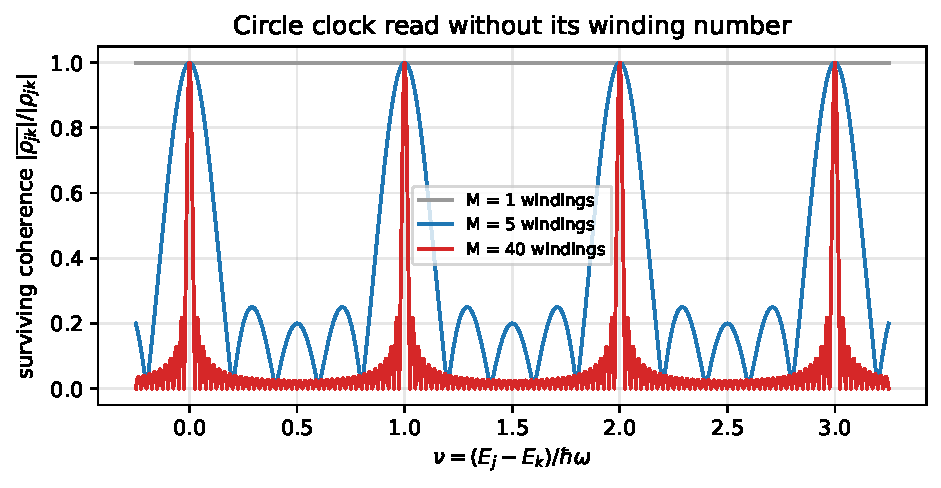
\includegraphics[width=0.62\linewidth]{figures/fig2_winding.pdf}
  \caption{Coherence surviving winding marginalization, $|D_M(\nu)|$ of Eq.~\eqref{eq:winding}, as a function of $\nu=(E_j-E_k)/\hbar\omega$. As the number of uncounted windings $M$ grows, only commensurate energy differences survive.}
  \label{fig:winding}
\end{figure}
\begin{figure}[t]
  \centering
  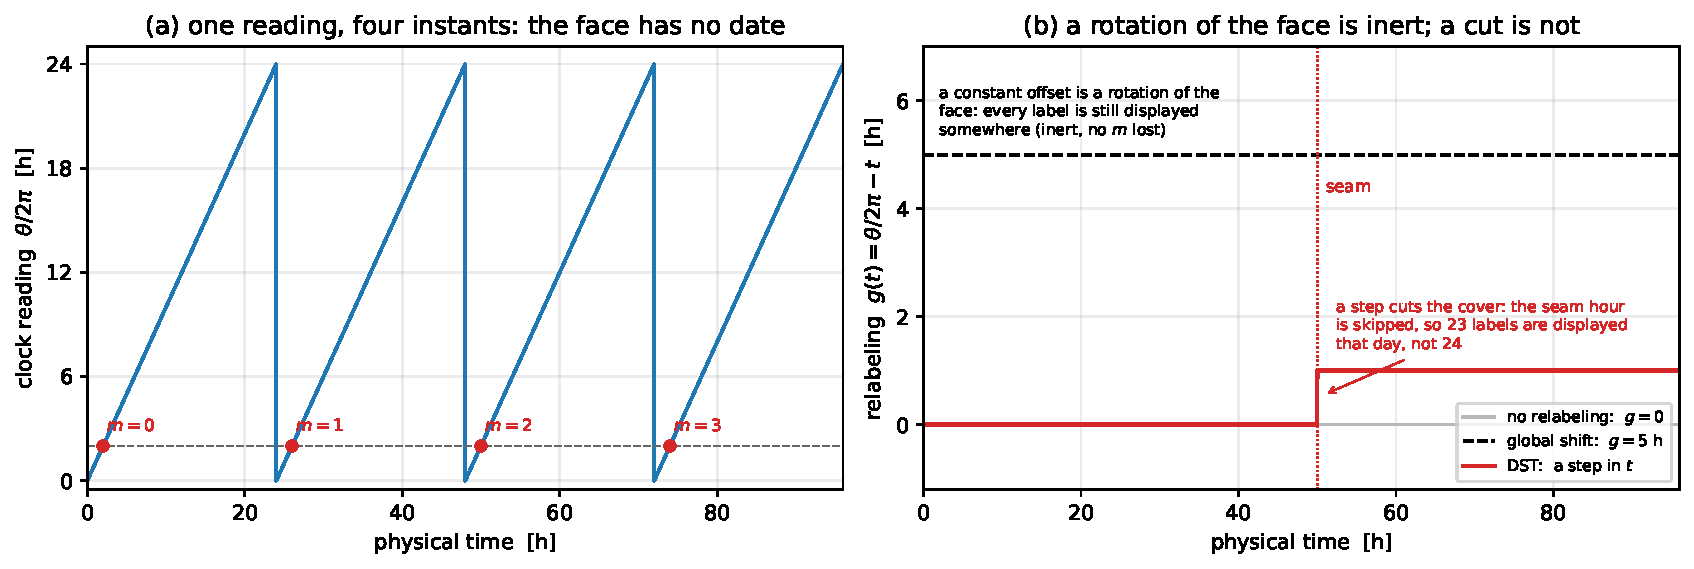
\includegraphics[width=\linewidth]{figures/fig_cover.pdf}
  \caption{The clock face has no date. (a)~The reading map $\theta/2\pi$ is a covering of the line onto the circle: a single reading, 2~A.M., corresponds to four distinct instants in four days, labelled by the winding number $m=0,1,2,3$ that Proposition~\ref{prop:winding} marginalizes over. (b)~The relabeling $g(t)=\theta/2\pi-t$ makes the distinction sharp. A constant offset is a rotation of the face, physically inert. A step applied after a seam --- daylight saving time --- cuts the cover and deletes one label from that day: the clock displays 23 distinct hours instead of 24, and one reading exists at no physical time at all. Both panels are computed in \texttt{scripts/make\_figures.py}.}
  \label{fig:cover}
\end{figure}
\begin{figure}[t]
  \centering
  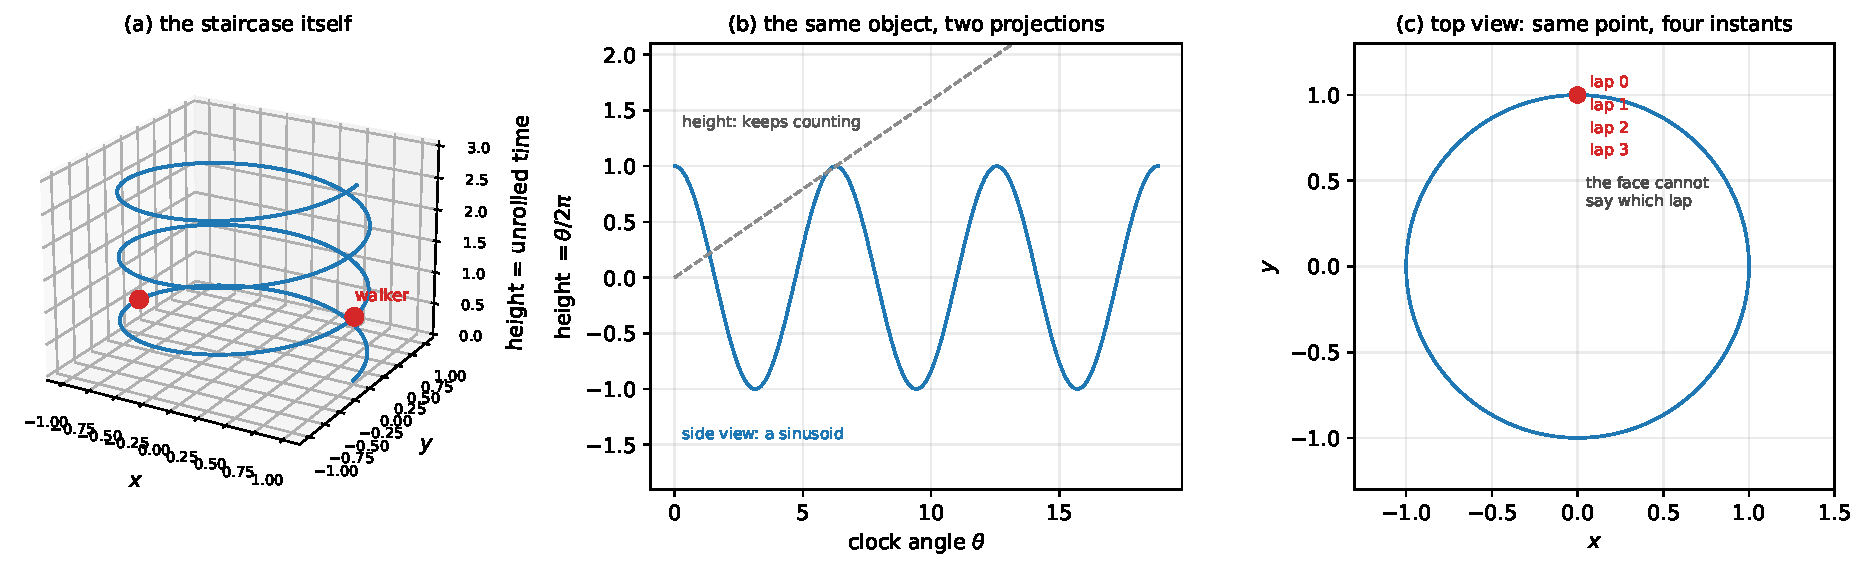
\includegraphics[width=\linewidth]{figures/fig_staircase.pdf}
  \caption{The clock as a staircase. (a)~A uniform staircase is a helix: walking along it is unrolled time (the universal cover), each step is a tick. (b)~The same object in two projections: from the side it is a sinusoid, the oscillation a clock represents, while the height keeps counting. (c)~From above it is a circle, and a given point of the face is reached once per lap with no record of which lap --- the winding number that Proposition~\ref{prop:winding} marginalizes over. Line, circle and oscillation are three projections of one object, and a projection is a choice of what to forget.}
  \label{fig:staircase}
\end{figure}

\begin{figure}[t]
  \centering
  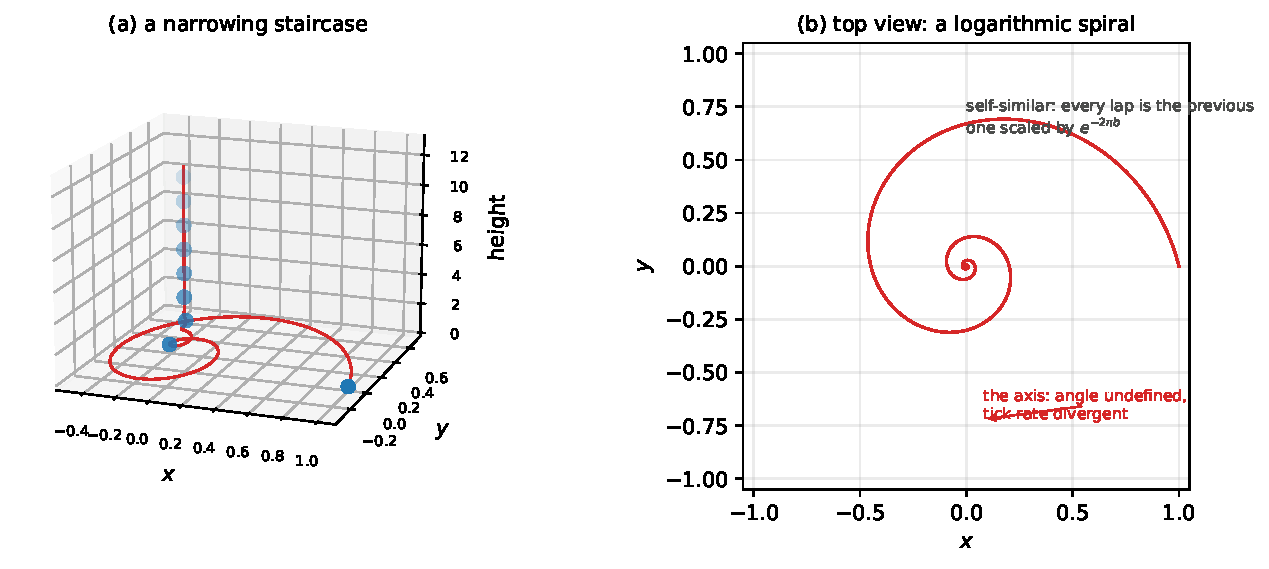
\includegraphics[width=0.92\linewidth]{figures/fig_staircase_conical.pdf}
  \caption{Why there is a vanishing point. (a)~A staircase that narrows as it climbs is a conical helix; a walker on it fades out of the projection as the radius shrinks. (b)~Its top view is a logarithmic spiral, self-similar under a scale factor per lap, with a turn rate that diverges at the axis. The apparent "centre" into which the walker disappears is a fixed point of the projection, where the angle is undefined, not a place that anything reaches. Both panels are computed in \texttt{scripts/make\_figures.py}.}
  \label{fig:staircaseconical}
\end{figure}

\subsection{Operational compactifications}
When one works directly on a compact clock, incommensurability is handled either by (1)~a \emph{spectral window}: normalizable states $|\Psi_\epsilon\rangle\propto f(\Cop/\epsilon)|\eta\rangle$ with $f$ peaked at zero, satisfying $\langle\Cop^2\rangle\lesssim\epsilon^2$; or (2)~a finite Pegg--Barnett clock~\cite{PeggBarnett1989} $\Hil_C^{(N)}=\C^N$ with orthonormal phase states
\begin{equation}
  |\theta_k^{(N)}\rangle=\frac{1}{\sqrt N}\sum_{n=0}^{N-1}e^{in\theta_k}|n\rangle,\qquad \theta_k=\frac{2\pi k}{N}.
  \label{eq:pb}
\end{equation}

\begin{remark}[Sign conventions and semi-bounded clocks]
\label{rem:signs}
The overall sign of a constraint is immaterial, but the \emph{relative} sign of clock and system energies is not. In Eq.~\eqref{eq:circ_constraint} the clock enters with the opposite sign to the system, so that a clock with $\Spec(\Nop)=\N_0$ pairs with system energies $E_k=\hbar\omega n_k\ge0$ and conditioning on the bra $\pbra{\theta}$ of Sec.~\ref{sec:povm} gives forward evolution. Because a semi-bounded clock covers only part of the real line, only system energies in a corresponding window (after a constant shift of $\Hs$) are represented. The Hardy restriction below is therefore a \emph{selection rule}, and this is the mechanism behind the positive-frequency selection of Sec.~\ref{sec:kg}.
\end{remark}

%==============================================================================
\section{The covariant clock POVM}
\label{sec:povm}
%==============================================================================

Let the physical clock be the Hardy space $\Hil_C=H^2(S^1)$ spanned by $\{|n\rangle\}_{n\ge0}$ with $\widehat H_C=\hbar\omega\Nop$, $\Spec(\Nop)=\N_0$. Following Holevo~\cite{Holevo1982} define the generalized vectors
\begin{equation}
  \pket{\theta}=\sum_{n=0}^{\infty}e^{in\theta}|n\rangle,\qquad\theta\in[0,2\pi).
  \label{eq:holevo}
\end{equation}
Because the sum starts at $n=0$ these vectors are not orthogonal. Their overlap is the boundary value of the Szeg\H{o} kernel,
\begin{equation}
  \pbra{\theta}\theta')=\sum_{n=0}^\infty e^{in(\theta'-\theta)}=\frac{1}{1-e^{i(\theta'-\theta+i0^+)}}
  =\pi\,\delta_{2\pi}(\theta'-\theta)+\frac12+\frac i2\,\mathrm{P.V.}\cot\frac{\theta'-\theta}{2},
  \label{eq:szego}
\end{equation}
where the delta function is produced by the $+i0^+$ prescription (Sokhotski--Plemelj) and must not be added a second time.

\begin{proposition}[Covariant circular clock POVM]
\label{prop:povm}
$E(\Delta)=\int_\Delta E(d\theta)$, $E(d\theta)=\frac{1}{2\pi}\pket{\theta}\pbra{\theta}\,d\theta$, defines a POVM on the Borel sets of $S^1$ with:
(1)~positivity, $\langle\chi|E(\Delta)|\chi\rangle=\int_\Delta\frac{d\theta}{2\pi}|\pbra{\theta}\chi\rangle|^2\ge0$;
(2)~completeness, $E(S^1)=I_C$;
(3)~covariance, $U(\phi)E(\Delta)U^\dagger(\phi)=E(\Delta\oplus\phi)$ with $U(\phi)=e^{i\phi\Nop}$;
(4)~the Pegg--Barnett PVMs $E^{(N)}(\Delta)=\sum_{\theta_k\in\Delta}|\theta_k^{(N)}\rangle\langle\theta_k^{(N)}|$ converge weakly to $E(\Delta)$ on finitely supported vectors as $N\to\infty$.
It is not projection valued, which is how it is compatible with Pauli's theorem~\cite{Holevo1982,BuschGrabowskiLahti1995}.
\end{proposition}

\begin{proof}
(1) is immediate. For (2), with $|\chi\rangle=\sum_nc_n|n\rangle$, $\int_0^{2\pi}\frac{d\theta}{2\pi}\sum_{n,m}c_n^*c_me^{i(n-m)\theta}=\sum_n|c_n|^2$; polarization gives $E(S^1)=I_C$. For (3), $U(\phi)\pket{\theta}=\pket{\theta+\phi}$ and the measure is translation invariant. For (4), $\langle\chi|E^{(N)}(\Delta)|\eta\rangle$ is a Riemann sum of $\int_\Delta\frac{d\theta}{2\pi}\langle\chi\pket{\theta}\pbra{\theta}\eta\rangle$ once $N$ exceeds the support.
\end{proof}

\begin{remark}
On a twisted fibre $\Hil_\kappa$ of Proposition~\ref{prop:zak} the same construction with $\pket{\theta}_\kappa=\sum_{n\ge0}e^{i(n+\kappa/2\pi)\theta}|n+\kappa/2\pi\rangle$ gives a covariant POVM with identical properties; the clock ``number'' then takes values in $\N_0+\kappa/2\pi$.
\end{remark}

%==============================================================================
\section{The quadrature conjecture and the tri-fold conditional structure}
\label{sec:quadrature}
%==============================================================================

\begin{definition}[Tri-fold quadrature]
\label{def:trifold}
Let $|\Psi\rangle\in\Hil_C\otimes\Hil_S$, let $E(d\theta)$ be the clock POVM and let $|\Psi(\theta)\rangle=(\pbra{\theta}\otimes I_S)|\Psi\rangle$. Define
\begin{align}
  &\text{raw clock marginal:} && M_\Psi(\theta)=\tfrac{1}{2\pi}\|\Psi(\theta)\|^2, \label{eq:marginal}\\
  &\text{joint quadrature:} && J_\Psi(\theta,F)=\tfrac{1}{2\pi}\langle\Psi(\theta)|F|\Psi(\theta)\rangle,\quad 0\le F\le I_S, \label{eq:joint}\\
  &\text{conditional state:} && \rho_S(\theta)=\frac{|\Psi(\theta)\rangle\langle\Psi(\theta)|}{\|\Psi(\theta)\|^2},\qquad P_\Psi(F|\theta)=\frac{J_\Psi(\theta,F)}{M_\Psi(\theta)}=\Tr[\rho_S(\theta)F]. \label{eq:conditional}
\end{align}
\end{definition}

\paragraph*{Where the circle is squared.}
Equation~\eqref{eq:marginal} is the precise step to which the title refers. The clock amplitudes $|\Psi(\theta)\rangle$ carry the $U(1)$ phases of Eq.~\eqref{eq:hopf}, and no measurement can see their common part. The quadratic map $\|\cdot\|^2$ removes that common phase and converts the \emph{relative} phases between clock levels, which are what $\pbra{\theta}$ reads out, into a nonnegative density over readings. Equations~\eqref{eq:joint}--\eqref{eq:conditional} apply the same squaring to the system, so that each reading carries a state. ``Squaring'' here means this quadratic (Born) map and nothing more; no relation to the classical compass-and-straightedge problem is implied.

\begin{conjecture}[Hilbert-space quadrature conjecture]
\label{conj:main}
In a closed quantum universe there is no primitive external time parameter. Temporal order and dynamics are generated by the universal wave function through the quadratic map $\Psi\mapsto(M_\Psi,J_\Psi,\rho_S)$ over a covariant clock POVM; classical time $t=\theta/\omega$ (with winding number counted, Sec.~II.D) is a derived semiclassical statistic of this structure.
\end{conjecture}

\begin{theorem}[Conditional Schr\"odinger dynamics; cf.~\cite{PageWootters1983,SmithAhmadi2019,Hohn2021}]
\label{thm:schrodinger}
Let $|\Psi\rangle$ satisfy Eq.~\eqref{eq:circ_constraint} with $\Hil_C=H^2(S^1)$ and system energies $E_k=\hbar\omega n_k$, $n_k\in\N_0$. Then (i)~$M_\Psi(\theta)=1/2\pi$; (ii)~$\rho_S(t):=\rho_S(\omega t)=|\psi(t)\rangle\langle\psi(t)|$ with $i\hbar\,\partial_t|\psi(t)\rangle=\Hs|\psi(t)\rangle$.
\end{theorem}

\begin{proof}
The constraint restricts $|\Psi\rangle=\sum_k\alpha_k|n_k\rangle|E_k\rangle$, $\sum_k|\alpha_k|^2=1$. Then $|\Psi(\theta)\rangle=\sum_k\alpha_ke^{-iE_k\theta/\hbar\omega}|E_k\rangle$, whose norm is $1$, giving (i); differentiating with $\partial_\theta=\omega^{-1}\partial_t$ gives (ii).
\end{proof}

Theorem~\ref{thm:schrodinger} has a simple reading in these terms. An exact constraint state squares the circle into a \emph{flat} measure (i): every reading is equally weighted, so the universe has dynamics (ii) but no preferred moment. This is the PW answer to ``frozen time'': what is frozen is the marginal, not the conditional evolution. This is the standard PW result expressed with a covariant POVM; it holds equally on a twisted fibre (any $E_k\in\hbar\omega(\N_0+\kappa/2\pi)$) and on the universal cover. It is verified numerically in Appendix~\ref{app:numerics}.

\begin{proposition}[Peaked clocks from spectral windows]
\label{prop:window}
For $w\in\mathcal S(\R)$ with $\int|w|^2dt=1$ and temporal width $\Delta T$, let $|\Psi_w\rangle=\int dt\,w(t)|t\rangle\otimes e^{-i\Hs t/\hbar}|\psi_0\rangle$. Then $\|\Cop_{\rm univ}\Psi_w\|=\hbar\|w'\|_{L^2}$ ($=\hbar/2\Delta T$ for a Gaussian), $M_{\Psi_w}(t)=|w(t)|^2$, and the conditional state is $e^{-i\Hs t/\hbar}|\psi_0\rangle$ on the support of $w$.
\end{proposition}

\begin{proof}
$(-i\hbar\,d/dt+\Hs)[w(t)e^{-i\Hs t/\hbar}\psi_0]=-i\hbar w'(t)e^{-i\Hs t/\hbar}\psi_0$; take norms. The rest follows from $\langle t|\Psi_w\rangle=w(t)e^{-i\Hs t/\hbar}\psi_0$.
\end{proof}

Unitarity of the conditional evolution here holds by construction; the content of the proposition is the trade-off between a peaked marginal and an approximate constraint. Exact constraint states have uniform marginals (Theorem~\ref{thm:schrodinger}); peaked clocks require $\|\Cop\Psi\|\neq0$. This answers the familiar objection that a stationary universe cannot display a ``present moment''.

\subsection{Wigner--Weyl quadrature}
For $\Hil_S=L^2(\R^n)$ let $\psi(q,\theta)=(\pbra{\theta}\otimes\langle q|)|\Psi\rangle$ and define the conditional Wigner function
\begin{equation}
  W_\Psi(q,p;\theta)=\frac{1}{(2\pi\hbar)^n}\int d^ny\,e^{-ip\cdot y/\hbar}\,\psi\!\left(q+\tfrac y2,\theta\right)\psi^*\!\left(q-\tfrac y2,\theta\right).
  \label{eq:wigner}
\end{equation}
Then $\int d^nq\,d^np\,W_\Psi=2\pi M_\Psi(\theta)$, and under Theorem~\ref{thm:schrodinger}, $\omega\,\partial_\theta W_\Psi=\{\!\{H_S,W_\Psi\}\!\}_{\rm Moyal}\to\{H_S,W_\Psi\}_{\rm PB}$ as $\hbar\to0$. Geometrically, a single quadratic map acts on both factors. On the clock factor it produces the temporal weight $2\pi M_\Psi(\theta)$; on the system factor it produces a quasi-distribution on the classical phase space $\R^{2n}$, whose $\theta$-flow becomes the Hamiltonian flow as $\hbar\to0$. The circle supplies the ordering parameter, and the squared system amplitudes supply the arena in which classical motion along it takes place. Two cautions apply. First, $\R^{2n}$ is the phase space of the \emph{system}; it is not the projective space $\mathbb P(\Hil)=S(\Hil)/U(1)$ of Eq.~\eqref{eq:hopf}, which is a K\"ahler manifold of real dimension $2(\dim\Hil-1)$. Second, $W_\Psi$ can be negative, so ``distribution'' is meant in the quasi-probability sense.

%==============================================================================
\section{Finite-clock corrections}
\label{sec:finite}
%==============================================================================

Two physically different imperfections must be distinguished.

\paragraph*{A remark on ``clock energy spread''.}
In an exact constraint state the clock's energy distribution is fixed by the system's: for $|\Psi\rangle=\sum_k\alpha_k|n_k\rangle|E_k\rangle$ it is $\{|\alpha_k|^2\}$. Dressing each clock level with a wave packet, $\sum_ng(n)|n+n_k\rangle$, contributes only a common factor $\hat g(\theta)$ to $|\Psi(\theta)\rangle$ and produces no dephasing. Dephasing requires either an unsharp \emph{readout} or noise in, or interaction with, the clock~\cite{SmithAhmadi2019}.

\subsection{Unsharp readout: a static effect}
\begin{proposition}[Unsharp covariant readout]
\label{prop:unsharp}
Let the clock be read with the smeared covariant POVM $E_\sigma(d\theta)=d\theta\int d\theta'\,G_\sigma(\theta-\theta')\,\frac{1}{2\pi}\pket{\theta'}\pbra{\theta'}$, with $G_\sigma$ a (wrapped) Gaussian of width $\sigma_\theta$. For an exact constraint state,
\begin{equation}
  \rho_S^{\sigma}(\theta)=\int d\phi\,G_\sigma(\phi)\,\rho_S(\theta-\phi),\qquad
  \rho^{\sigma}_{jk}(\theta)=\rho_{jk}(\theta)\,e^{-\nu_{jk}^2\sigma_\theta^2/2}=\rho_{jk}(\theta)\,e^{-\omega_{jk}^2\sigma_t^2/2},
  \label{eq:static}
\end{equation}
with $\nu_{jk}=(E_j-E_k)/\hbar\omega$, $\omega_{jk}=(E_j-E_k)/\hbar$ and $\sigma_t=\sigma_\theta/\omega$ (the wrapped-Gaussian correction is exponentially small for $\sigma_\theta\ll\pi$). The suppression is \emph{independent of $\theta$}.
\end{proposition}

\begin{proof}
$E_\sigma$ is a convex mixture of shifted copies of $E$ and hence a covariant POVM. Since $M_\Psi$ is uniform the smeared marginal is uniform, and the unnormalized conditional state is the $G_\sigma$-average of $|\Psi(\theta')\rangle\langle\Psi(\theta')|$. In the energy basis this multiplies $\rho_{jk}$ by the characteristic function of $G_\sigma$ at $\nu_{jk}$.
\end{proof}

With a Fourier-limited resolution $\sigma_t\simeq\hbar/(2\Delta E_C)$ the factor is $\exp[-(E_j-E_k)^2/(8\Delta E_C^2)]$, which is negligible for any macroscopic clock (Sec.~\ref{sec:experiment}).

\subsection{Diffusive clock error: the Lindblad form}
\begin{assumption}[Diffusive clock]
\label{ass:diffusive}
The timing error of the clock, relative to an ideal relational clock, is Gaussian with variance growing linearly, $\sigma_t^2(t)=\sigma_0^2+T_Ct$, with a phenomenological clock-diffusion time $T_C$.
\end{assumption}

\begin{proposition}[Double-commutator master equation under Assumption~\ref{ass:diffusive}]
\label{prop:lindblad}
Let $\rho_S^{\rm obs}(t)=\int d\tau\,G_{\sigma_t(t)}(\tau)\,U(t+\tau)\rho_S(0)U^\dagger(t+\tau)$. Then (i)~to second order in $\sigma_t$, $\rho_S^{\rm obs}(t)=U(t)\big[\rho_S(0)-\frac{\sigma_t^2}{2\hbar^2}[\Hs,[\Hs,\rho_S(0)]]\big]U^\dagger(t)+\mathcal O(\sigma_t^4)$; (ii)~exactly, $\rho^{\rm obs}_{jk}(t)=\rho_{jk}(0)e^{-i\omega_{jk}t-\omega_{jk}^2\sigma_t^2(t)/2}$; (iii)~for $\sigma_0=0$, $\rho_S^{\rm obs}$ obeys the GKSL equation
\begin{equation}
  \frac{d\rho_S}{dt}=-\frac{i}{\hbar}[\Hs,\rho_S]-\frac{T_C}{2\hbar^2}[\Hs,[\Hs,\rho_S]],\qquad
  \Gamma_{jk}=\frac{T_C}{2\hbar^2}(E_j-E_k)^2,
  \label{eq:lindblad}
\end{equation}
with the single Hermitian jump operator $L=\sqrt{T_C}\,\Hs/\hbar$.
\end{proposition}

\begin{proof}
(i) follows from expanding $U(\tau)\rho U^\dagger(\tau)$ to second order and using $\int G\tau=0$, $\int G\tau^2=\sigma_t^2$. (ii) is the Gaussian Fourier transform. Differentiating (ii) with $\sigma_t^2=T_Ct$ gives $\dot\rho_{jk}=(-i\omega_{jk}-\frac{T_C}{2}\omega_{jk}^2)\rho_{jk}$, which is Eq.~\eqref{eq:lindblad} in the energy basis since $[\Hs,[\Hs,|E_j\rangle\langle E_k|]]=\hbar^2\omega_{jk}^2|E_j\rangle\langle E_k|$; finally $-\frac12[H,[H,\rho]]=H\rho H-\frac12\{H^2,\rho\}$.
\end{proof}

\begin{remark}
Equation~\eqref{eq:lindblad} is the real-clock master equation of Egusquiza \emph{et al.}~\cite{Egusquiza1999}; it is also the structure of Milburn's intrinsic decoherence~\cite{Milburn1991} and of the Gambini--Porto--Pullin mechanism~\cite{Gambini2004} (which uses a different, non-linear growth of $\sigma_t^2$). Within standard quantum mechanics $T_C$ is set by the measured phase noise of the clock. A common heuristic, $T_C\sim\hbar/\Delta E_C$, is only a dimensional estimate: it is not implied by Proposition~\ref{prop:unsharp}, which gives a static effect, and it is not derived here. The conjecture acquires empirical content beyond standard quantum mechanics only if it supplies an independent law for $T_C$.
\end{remark}

Figure~\ref{fig:conditioning} illustrates Theorem~\ref{thm:schrodinger} and Propositions~\ref{prop:unsharp}--\ref{prop:lindblad} computed from an explicit bipartite state.

\begin{figure}[t]
  \centering
  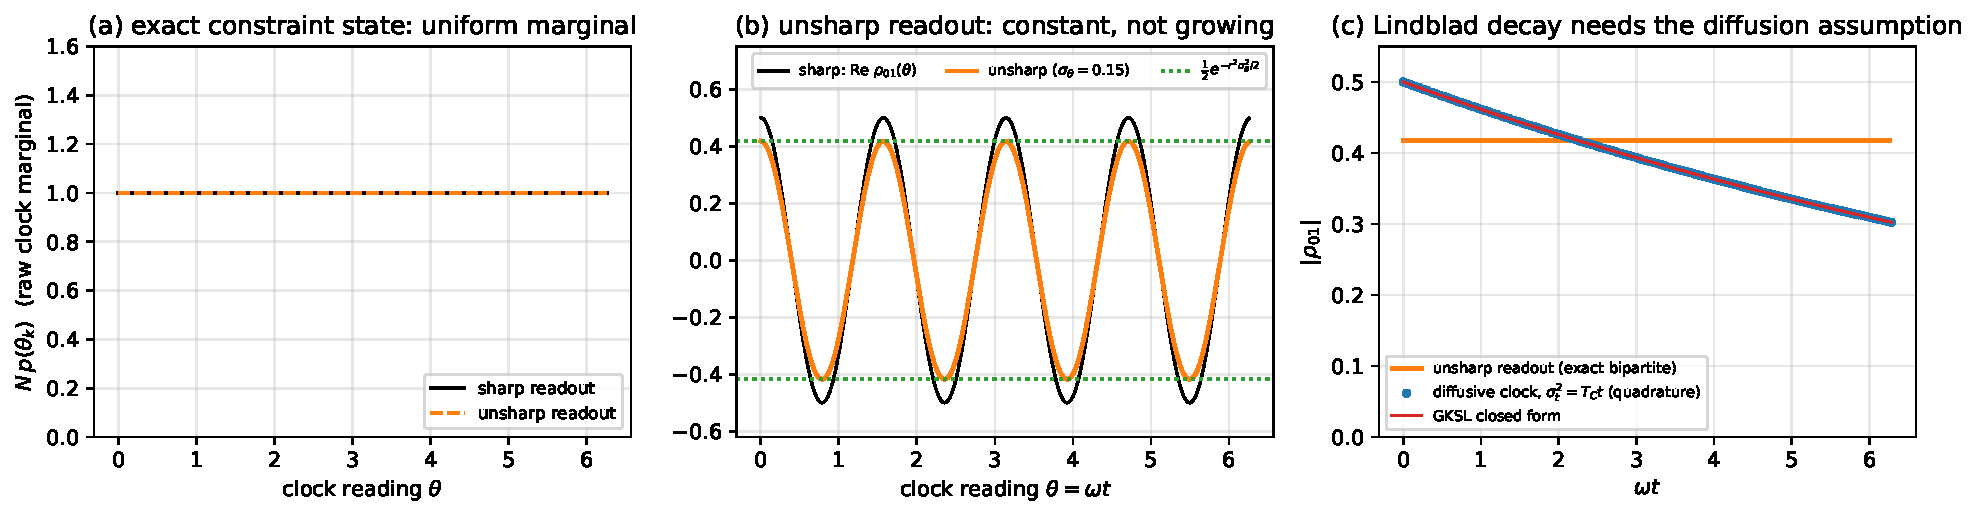
\includegraphics[width=\linewidth]{figures/fig1_conditioning.pdf}
  \caption{Exact bipartite computation in $\C^{256}\otimes\C^2$ with system gap $r=4$ clock quanta. (a)~Raw clock marginal is uniform (Theorem~\ref{thm:schrodinger}). (b)~Unsharp readout ($\sigma_\theta=0.15$) suppresses the conditional coherence by the constant factor $e^{-r^2\sigma_\theta^2/2}$ (Proposition~\ref{prop:unsharp}). (c)~Exponential decay arises only under the diffusive Assumption~\ref{ass:diffusive}; direct quadrature of the smearing channel coincides with the GKSL solution (Proposition~\ref{prop:lindblad}).}
  \label{fig:conditioning}
\end{figure}

\subsection{How many levels does a clock need?}
\label{sec:levels}
The preceding two subsections describe imperfections of a clock that is already built. A different and purely kinematic question is how accurately a finite, equally spaced clock can represent a system whose energies are arbitrary, and for how long. This is a design question, it is independent of the conjecture, and it has a sharper answer than one might expect.

\paragraph*{Setup.}
Let the system have energies $E_1<\dots<E_d$ with weights $p_j=|\alpha_j|^2$, and let the clock have $N$ equally spaced levels, so that level $j$ is represented by the energy $q_j\hbar\omega$ with integer label $q_j\in\{0,\dots,N-1\}$. The mismatch is $\delta_j=E_j-q_j\hbar\omega$, and its weighted variance $\operatorname{Var}_p(\delta)=\sum_jp_j(\delta_j-\bar\delta)^2$ controls how fast the conditioned state drifts away from the exact one, by a bound recorded below.

\begin{lemma}[Energy-mismatch fidelity bound]
\label{lem:fidbound}
Let $A(t)=\sum_jp_je^{-i\delta_jt/\hbar}$ be the overlap between the exact conditional state and the state produced by the mismatched clock. Then $F(t)=|A(t)|^2\ge\max\{0,1-t^2\operatorname{Var}_p(\delta)/\hbar^2\}$.
\end{lemma}
\begin{proof}
$1-F=2\sum_{j<k}p_jp_k[1-\cos((\delta_j-\delta_k)t/\hbar)]\le t^2\hbar^{-2}\sum_{j<k}p_jp_k(\delta_j-\delta_k)^2$, using $1-\cos x\le x^2/2$, and the last sum equals $\operatorname{Var}_p(\delta)$. Both quantities are invariant under a common energy offset.
\end{proof}

\paragraph*{The design problem.}
Minimising $\operatorname{Var}_p(\delta)$ over the scale $\hbar\omega>0$ for a fixed assignment $q$ is a weighted least-squares fit, so the optimum is explicit: $\hbar\omega^\star=C_{Eq}/V_q$ and $V^\star(q)=V_E-C_{Eq}^2/V_q=V_E(1-\varrho^2)$, with $V_E,V_q$ the weighted variances of the energies and labels, $C_{Eq}$ their weighted covariance and $\varrho$ their weighted correlation. The design problem is therefore to \emph{choose the integer regressor $q$, distinct and increasing inside the allowed range, that maximises its squared correlation with the spectrum}. Write $V^\star_N$ for its minimum over all such $q$, and $R=E_d-E_1$ for the range that must be resolved.

\begin{proposition}[Universal bound]
\label{prop:universalb}
For any spectrum, any weights and any $N\ge2$,
\begin{equation}
  V^\star_N\le\frac{R^2}{4(N-1)^2},
  \qquad\text{hence}\qquad
  T(\varepsilon)\ge\frac{2(N-1)\sqrt{\varepsilon}}{R}
  \label{eq:universal}
\end{equation}
is a time up to which the infidelity is guaranteed to stay below $\varepsilon$ (Lemma~\ref{lem:fidbound}).
\end{proposition}
\begin{proof}
Round each shifted energy to its nearest label. Then $|\delta_j|\le\hbar\omega/2$, so the $\delta_j$ span at most $\hbar\omega$ and Popoviciu's inequality, $\operatorname{Var}\le(\text{range})^2/4$, gives $\operatorname{Var}_p(\delta)\le(\hbar\omega)^2/4$. The largest label is $R/\hbar\omega$, which must fit in $N-1$ steps, so $\hbar\omega\ge R/(N-1)$. Insert into Lemma~\ref{lem:fidbound} and solve for $t$.
\end{proof}

This is unconditional --- no number theory, no assumption on the spectrum --- but it is far from tight: for incommensurate spectra the optimum beats Eq.~\eqref{eq:universal} by two to five orders of magnitude, and that gap is where the physics of the problem lies.

\begin{proposition}[Three-level closed form and the $N^{-4}$ law]
\label{prop:closedform}
For $d=3$ with energies $(0,\mathcal{E},\mathcal{E}(1+r))$ and uniform weights, and labels $(0,q,p)$,
\begin{equation}
  V^\star(q,p)=\frac{(p-rq)^2}{(p+q)^2+(2q-p)^2+(2p-q)^2}\,\mathcal{E}^2 .
  \label{eq:closedform}
\end{equation}
The numerator is the rational-approximation error of the gap ratio $r$; the denominator is $9V_E/\mathcal{E}^2=(p+q)^2+(2q-p)^2+(2p-q)^2$, which equals $27V_E/\mathcal{E}^2$ up to corrections of order $1/q$. Consequently, writing $|r-p/q|=\kappa/q^2$ along the convergents of $r$ and using $q\simeq p/r$,
\begin{equation}
  V^\star_N\;\simeq\;\frac{\kappa(r)^2r^4}{27V_E}\,N^{-4},
  \qquad
  T(\varepsilon)\;\simeq\;\frac{N^2}{\kappa}\sqrt{\frac{27V_E\,\varepsilon}{r^4}} .
  \label{eq:nfour}
\end{equation}
\end{proposition}
\begin{proof}
Write $s=p/q$ and $u_x=\frac13\big(-(1+x),\,2-x,\,2x-1\big)$. Both centred vectors lie in the two-dimensional subspace orthogonal to $(1,1,1)$, with $v_E=\mathcal{E}u_r$ for the energies and $v_q=qu_s$ for the labels. A direct computation gives $u_r\wedge u_s=\frac{s-r}{3}(1,1,1)$, hence $|v_E\wedge v_q|^2=\mathcal{E}^2(p-rq)^2/3$, and $|v_q|^2=q^2\big[(1+s)^2+(2-s)^2+(2s-1)^2\big]/9$. Since $1-\varrho^2=\sin^2\theta=|v_E\wedge v_q|^2/(|v_E|^2|v_q|^2)$ and $V^\star=\frac13|v_E|^2\sin^2\theta$, substituting and cancelling $q$ gives Eq.~\eqref{eq:closedform}. The asymptotics follow by inserting $|r-p/q|=\kappa/q^2$ and $q\simeq p/r$.
\end{proof}

The content of Eq.~\eqref{eq:nfour} is that clock design is \emph{simultaneous Diophantine approximation}: the cost is quadratic in the rational-approximation error, so the variance falls four powers of $N$ faster than the rounding argument of Proposition~\ref{prop:universalb} predicts, and the guaranteed time horizon grows like $N^2$. The optimal labels are the convergent denominators of the gap ratio, and the constant is set by $\kappa(r)=\liminf q^2|r-p/q|$. Hurwitz's theorem bounds this quantity from above by $1/\sqrt5$, with equality for the golden ratio and its continued-fraction relatives~\cite{Hurwitz1891}, so the golden ratio shows the slowest power law available. The \emph{constant} also carries the factor $r^4/V_E(r)$, so an extremal statement over all spectra does not follow from Hurwitz alone; among the spectra we have examined the golden ratio does give the slowest decay, and we state that as a numerical finding rather than a theorem. At Fibonacci labels the predicted constant is $\varphi^4/(135V_E)=0.1142350$, which we verify to $3\times10^{-8}$.

\begin{remark}[Scope and numerics]
\label{rem:scopenumerics}
Equation~\eqref{eq:closedform} requires three levels and uniform weights; with weights, or for $d\ge4$, the problem remains a weighted least-squares fit but no longer collapses to two vectors, and the general case is a lattice problem for which we have only a validated heuristic. The exponent $N^{-4}$ is likewise not universal: spectra built from powers of a single quadratic irrational show it in every dimension tested, whereas spectra with independent irrational ratios decay more slowly (numerically $N^{-3.1}$ for $(1,\sqrt2,\sqrt3)$ in the proportional family), which is the expected signature of approximation in $d-2$ dimensions. All of these statements are checked in the accompanying package: the closed form is confirmed against the density-matrix computation, the bound~\eqref{eq:universal} is confirmed with no violation for $N=4$--$128$ over five spectra, the golden-ratio constant is confirmed to $3\times10^{-8}$ in exact rational arithmetic, and the optimiser reproduces exhaustive enumeration for three and four levels. The design problem can be solved to $N=10^6$ in under a second. None of this bears on whether time is circular; it is what a finite clock can do regardless.
\end{remark}

\begin{figure}[t]
  \centering
  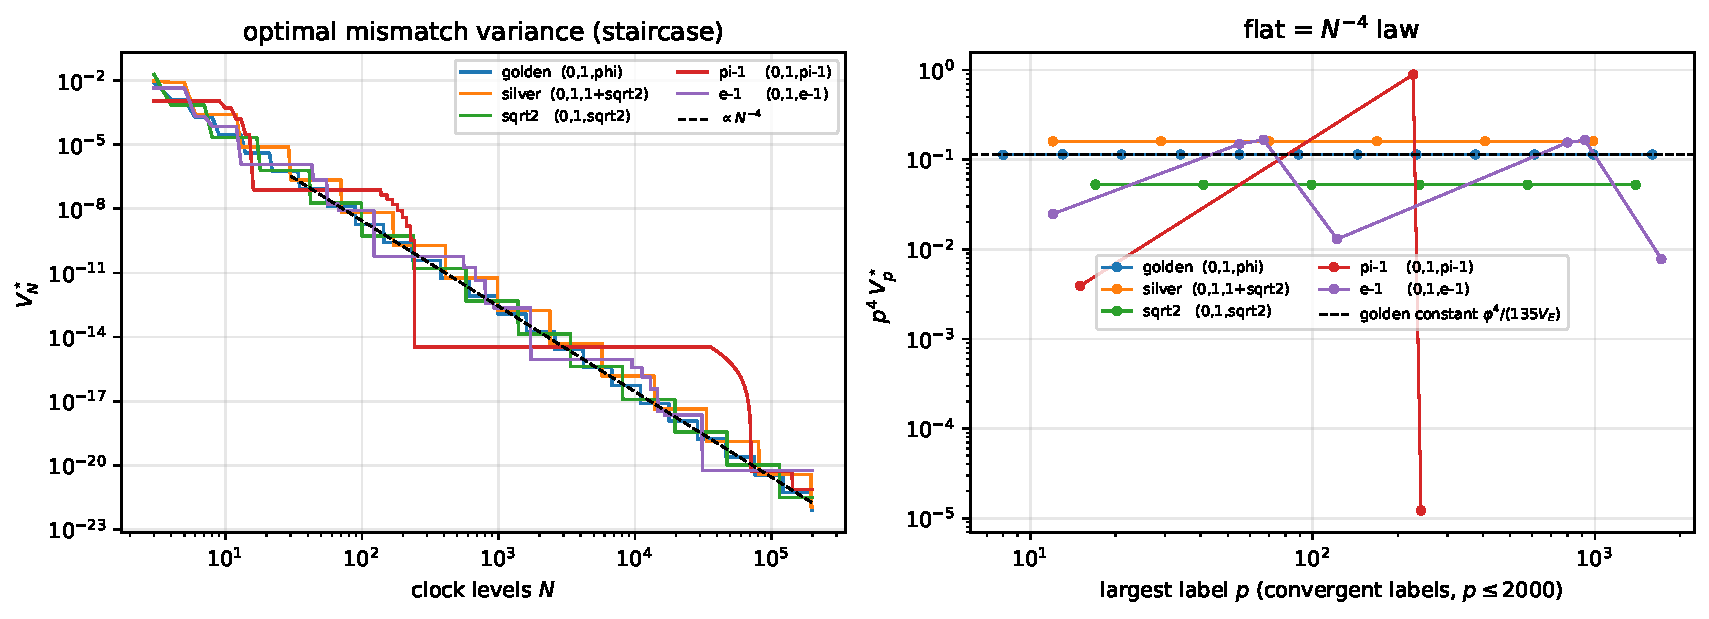
\includegraphics[width=\linewidth]{figures/fig5_clock_scaling.pdf}
  \caption{Finite-clock design for three-level spectra. (a)~The optimal mismatch variance $V^\star_N$ as a function of the number of clock levels: a staircase, because a larger clock helps only when it crosses a convergent of the gap ratio. The dashed line is the $N^{-4}$ envelope. (b)~$p^4V^\star_p$ at convergent labels, where the optimum re-equilibrates. Spectra built from a single badly approximable ratio sit on a flat envelope; the golden ratio attains the constant $\varphi^4/(135V_E)=0.1142$ (dashed), and the $\pi$-like spectrum dips below it at its exceptional convergent $355/113$. The universal bound~\eqref{eq:universal} is respected throughout but is two to five orders of magnitude above the curves.}
  \label{fig:clockscaling}
\end{figure}


%==============================================================================
\section{A laboratory test: circuit QED}
\label{sec:experiment}
%==============================================================================

Proposition~\ref{prop:lindblad} is the point at which the framework could, in principle, meet experiment, so we examine it immediately, before any relativistic extension. PW kinematics itself has been illustrated with entangled photons~\cite{Moreva2014}. A test of finite-clock effects must specify (a)~the null model, standard quantum mechanics with the measured clock noise, and (b)~which energies enter the rate.

Consider a transmon ($\omega_s/2\pi\approx5$~GHz) dispersively coupled to a resonator ($\omega_c/2\pi\approx6$~GHz) with $\widehat H_{\rm int}=\hbar\chi a^\dagger a|1\rangle\langle1|$, $\chi/2\pi\approx-1$~MHz, and use the resonator, prepared in a coherent state with $\Delta E_C=\hbar\omega_c\sqrt{\bar n}$, as the clock. Inserting the heuristic $T_C=\hbar/\Delta E_C$ into Eq.~\eqref{eq:lindblad} gives $\Gamma=(\Delta E)^2/(2\hbar\Delta E_C)$. Table~\ref{tab:cqed} and Fig.~\ref{fig:cqed} compare two identifications of $\Delta E$.

\begin{table}[h]
\caption{Model rate $\Gamma=(\Delta E)^2/(2\hbar\Delta E_C)$ for the circuit-QED parameters above (computed with \texttt{qtime.estimates}).}
\label{tab:cqed}
\begin{ruledtabular}
\begin{tabular}{ccccc}
$\bar n$ & $\Gamma$ for $\Delta E=\hbar\chi$ [s$^{-1}$] & implied time & $\Gamma$ for $\Delta E=\hbar\omega_s$ [s$^{-1}$] & implied $T_2$ \\
\colrule
$10$ & $166$ & $6.0$ ms & $4.1\times10^{9}$ & $0.24$ ns \\
$10^2$ & $52$ & $19$ ms & $1.3\times10^{9}$ & $0.76$ ns \\
$10^3$ & $17$ & $60$ ms & $4.1\times10^{8}$ & $2.4$ ns \\
$10^4$ & $5.2$ & $0.19$ s & $1.3\times10^{8}$ & $7.6$ ns \\
\end{tabular}
\end{ruledtabular}
\end{table}

\begin{enumerate}
\item With $\Delta E=\hbar\omega_s$, the qubit's actual energy gap relative to the resonator clock, the model predicts $T_2\lesssim10$~ns, whereas transmons routinely reach $T_2\sim0.1$--$1$~ms. \emph{The heuristic $T_C=\hbar/\Delta E_C$ with this identification is excluded.}
\item With $\Delta E=\hbar\chi$, rates of $5$--$170$~s$^{-1}$ lie one to three orders of magnitude below intrinsic qubit dephasing. Choosing $\chi$ amounts to working in a frame rotating at $\omega_s$, which is defined by an external laboratory clock; this identification needs a justification that the framework does not currently provide.
\item The static effect of Proposition~\ref{prop:unsharp}, with $\sigma_t=\hbar/2\Delta E_C$, is $1-\mathcal O(10^{-10})$ and unobservable.
\item Heterodyne detection realizes a smeared covariant phase POVM (the phase marginal of the Husimi function), not the canonical Holevo POVM; the smearing must be included in the null model.
\item The dispersive Hamiltonian is valid only for $\bar n\ll n_{\rm crit}=\Delta^2/4g^2\approx\Delta/4\chi$, with $\Delta=\omega_c-\omega_s$. For $\Delta/2\pi\approx1$~GHz and $\chi/2\pi\approx1$~MHz, $n_{\rm crit}\approx250$, so the rows $\bar n=10^3$--$10^4$ of Table~\ref{tab:cqed} lie outside the model's own regime. Sweeping $\bar n$ over three decades inside it requires $\chi/2\pi\lesssim2.5$~kHz, which lowers the $\chi$-rate to $10^{-3}$--$10^{-5}$~s$^{-1}$.
\end{enumerate}

\paragraph*{Protocol.} The intended discriminating experiment conditions the qubit coherence on a clock resonator whose phase noise is independently characterized. It holds the resonator linewidth $\kappa$, the temperature and the detuning fixed and sweeps the coherent-state amplitude, and hence $\Delta E_C\propto\sqrt{\bar n}$, at fixed $\chi$ inside the dispersive window. The signature of the heuristic is a residual dephasing rate scaling as $\bar n^{-1/2}$ after the null model has been subtracted. Two standard backgrounds have different $\bar n$ dependence. Measurement-induced dephasing grows linearly with $\bar n$ ($\propto\chi^2\bar n/\kappa$ for $\chi\ll\kappa$), and thermal-photon dephasing is set by the thermal occupation, independent of the drive. The opposite, decreasing trend is therefore a useful handle. Items~1 and~5 nevertheless bound what the protocol can reach. The $\omega_s$ identification is already excluded, and the $\chi$ identification gives rates far below intrinsic qubit dephasing once the dispersive constraint is respected. A null result would therefore constrain the heuristic $T_C\sim\hbar/\Delta E_C$, not the conjecture as such. The winding-marginalization effect (Proposition~\ref{prop:winding}) is a robust standard-quantum-mechanics prediction for cyclic clocks that any implementation should reproduce, but it does not discriminate the conjecture from standard quantum mechanics.

\begin{figure}[t]
  \centering
  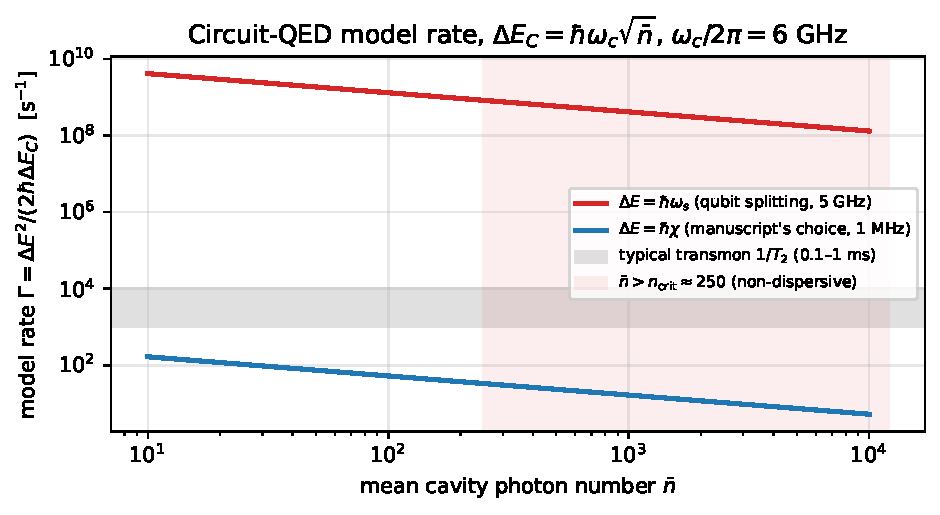
\includegraphics[width=0.62\linewidth]{figures/fig4_cqed.pdf}
  \caption{Model rate of Sec.~\ref{sec:experiment} versus mean photon number for the two identifications of the system energy gap, compared with typical transmon dephasing rates. Points with $\bar n\gtrsim n_{\rm crit}\approx250$ lie outside the dispersive regime (item~5).}
  \label{fig:cqed}
\end{figure}

%==============================================================================
\section{Consistency with thermal time}
\label{sec:modular}
%==============================================================================

\begin{proposition}[Modular flow for Gibbs Schmidt spectra]
\label{prop:modular}
Let $|\Psi\rangle=\sum_k\alpha_k|n_k\rangle|E_k\rangle$ with all $\alpha_k\neq0$, and let $\mathcal A_S=I_C\otimes B(\Hil_S)$ act on the closure of $\mathcal A_S|\Psi\rangle$. The modular operator is
\begin{equation}
  \Delta_\Psi=\rho_C^{-1}\otimes\rho_S,\qquad \sigma_s^\Psi(I\otimes A)=\Delta_\Psi^{is}(I\otimes A)\Delta_\Psi^{-is}=I\otimes\rho_S^{is}A\rho_S^{-is}.
  \label{eq:modular}
\end{equation}
If $|\alpha_k|^2=Z^{-1}e^{-\beta E_k}$, then $\sigma_s^\Psi(A)=e^{i\Hs t/\hbar}Ae^{-i\Hs t/\hbar}$ with $t=-\hbar\beta s$.
\end{proposition}

\begin{proof}
For the Tomita operator $S(I\otimes A)|\Psi\rangle=(I\otimes A^\dagger)|\Psi\rangle$ a direct computation in the Schmidt basis gives $S^*S=\rho_C^{-1}\otimes\rho_S$ (we have also checked this numerically by constructing $S$ from its definition; Appendix~\ref{app:numerics}). With $\rho_S=Z^{-1}e^{-\beta\Hs}$, $\rho_S^{is}A\rho_S^{-is}=e^{-is\beta\Hs}Ae^{is\beta\Hs}$, which equals the Heisenberg evolution at $t=-\hbar\beta s$.
\end{proof}

This is the KMS content of the thermal-time hypothesis~\cite{ConnesRovelli1994} restricted to the special case of a Gibbs entanglement spectrum. For non-Gibbs spectra modular flow and conditional (quadrature) time differ.

%==============================================================================
\section{Local relativistic regime: from flat spacetime to the horizon}
\label{sec:relativistic}
%==============================================================================

Sections~\ref{sec:relativistic} and~\ref{sec:cosmo} subject the conjecture to a progressive stress test, ordered by regime. Here the clock still lives in a fixed background: first flat spacetime (Klein--Gordon, Dirac, proper time), then a static gravitational field, and finally the near-horizon limit. Section~\ref{sec:cosmo} removes the background. Each result is either established (and attributed) or explicitly marked as heuristic.

\subsection{Klein--Gordon constraint and positive frequency}
\label{sec:kg}
With $\eta_{\mu\nu}=\mathrm{diag}(+,-,-,-)$, $\widehat P_0=\Pt/c$ and $\widehat M=mI+\widehat H_{\rm int}/c^2$, the mass-shell constraint factorizes as
\begin{equation}
  \left(\widehat P_\mu\widehat P^\mu-\widehat M^2c^2\right)=c^{-2}\,\Cop_+\Cop_-,\qquad
  \Cop_\pm=\Pt\pm\widehat H_{\rm rel},\quad \widehat H_{\rm rel}=\sqrt{c^2\widehat{\mathbf P}^2+\widehat M^2c^4}>0 .
  \label{eq:kg}
\end{equation}
\begin{proposition}[Semi-bounded clocks select positive frequency]
\label{prop:kg}
Restrict the universal-cover clock to the Hardy space of the line, i.e.\ to clock energy $\widehat H_C:=-\Pt\ge0$ (the line analogue of Remark~\ref{rem:signs}). Then $\ker\Cop_-$, on which $\widehat H_C=-\widehat H_{\rm rel}<0$, is annihilated, and conditional states on $\ker\Cop_+$ obey $i\hbar\,\partial_t\psi=\widehat H_{\rm rel}\psi$ with nonnegative density $|\langle\mathbf x|\psi(t)\rangle|^2$.
\end{proposition}
This is the standard positive-frequency (Newton--Wigner) restriction~\cite{NewtonWigner1949}, obtained here by the choice of a semi-bounded clock; the associated localization is not Lorentz covariant and spreads acausally~\cite{Hegerfeldt1974}. Working on the line rather than the circle avoids the commensurability issue for the continuous spectrum of $\widehat H_{\rm rel}$ (Corollary~\ref{cor:fibres}).

\subsection{Dirac constraint and Zitterbewegung}
For $\Hil_S=L^2(\R^3)\otimes\C^4$ the constraint $\Pt+\widehat H_D$, $\widehat H_D=c\bm\alpha\cdot\widehat{\mathbf P}+\beta mc^2$, has energies $\pm E_{\mathbf p}$. A semi-bounded clock as in Proposition~\ref{prop:kg} removes the negative-energy branch altogether (the Foldy--Wouthuysen sector~\cite{FoldyWouthuysen1950}), so no Zitterbewegung remains. Only for a two-sided (universal-cover) clock subject to Assumption~\ref{ass:diffusive} do the interference terms between branches decay, at rate $\Gamma_{\rm Zitt}=T_C(2E_{\mathbf p})^2/2\hbar^2\ge 2m^2c^4T_C/\hbar^2$; with the heuristic $T_C\sim\hbar/\Delta E_C$, $\Gamma_{\rm Zitt}\gtrsim2m^2c^4/(\hbar\Delta E_C)$.

\subsection{Internal proper-time quadrature}
For an internal Hardy clock $\widehat H_{\rm int}=\hbar\omega_0\Nop_{\rm int}$ carried by a particle of mass $m$,
\begin{equation}
  \widehat H_{\rm rel}=\widehat E_{\mathbf P}\otimes I+\widehat\gamma(\widehat{\mathbf P})^{-1}\otimes\hbar\omega_0\Nop_{\rm int}+\mathcal O\!\left(\widehat H_{\rm int}^2/mc^2\right),\qquad \widehat\gamma=\sqrt{1+\widehat{\mathbf P}^2/m^2c^2},
  \label{eq:proper}
\end{equation}
so the internal-clock reading conditioned on laboratory time satisfies $\langle\tau(t)\rangle=\langle\widehat\gamma^{-1}\rangle t$. A momentum superposition $c_1|\mathbf p_1\rangle+c_2|\mathbf p_2\rangle$ with the internal clock in a superposition of two levels $n,m$ shows the quantum twin-paradox modulation $|c_1|^4+|c_2|^4+2|c_1|^2|c_2|^2\cos[(n-m)\omega_0(\gamma_1^{-1}-\gamma_2^{-1})t]$~\cite{SmithAhmadi2020}. For a broad internal distribution $p_n$ the centre-of-mass visibility is $V(t)=|\sum_np_ne^{-in\omega_0\Delta t}|$ with $\Delta=\gamma_1^{-1}-\gamma_2^{-1}$. Because the internal spectrum is equally spaced, $V$ revives exactly with period $2\pi/(\omega_0|\Delta|)$; the Gaussian envelope $e^{-\Delta n^2\omega_0^2\Delta^2t^2/2}$ describes only the first collapse (Fig.~\ref{fig:interf}).

\begin{figure}[t]
  \centering
  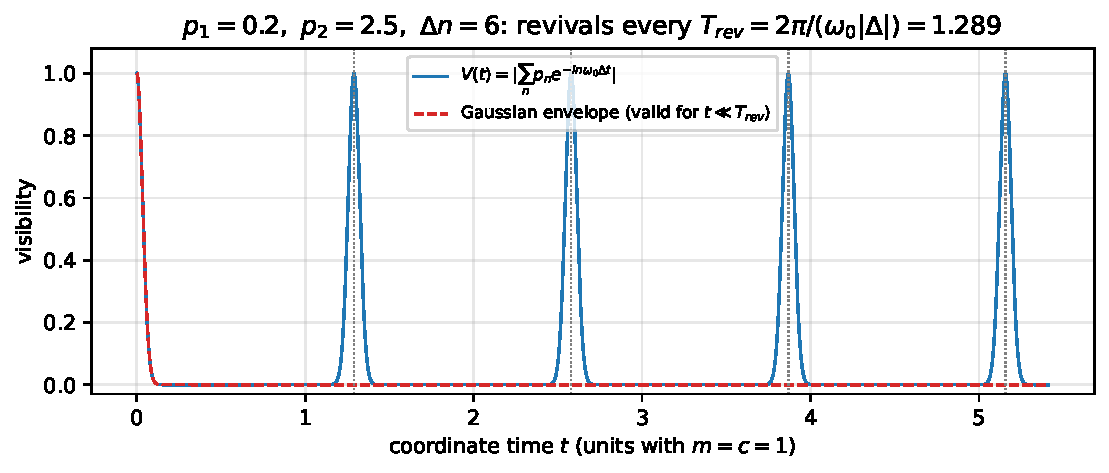
\includegraphics[width=0.7\linewidth]{figures/fig3_interferometer.pdf}
  \caption{Relativistic clock interferometer: exact visibility (solid) with full revivals, and the short-time Gaussian envelope (dashed).}
  \label{fig:interf}
\end{figure}

\subsection{Static spacetimes}
\label{sec:curved}
For $ds^2=N(\mathbf x)^2c^2dt^2-h_{ij}dx^idx^j$ (Schwarzschild exterior: $N=\sqrt{1-r_s/r}$, $r_s=2GM/c^2$), conditioning on an asymptotic clock gives the Killing Hamiltonian
\begin{equation}
  \widehat H_{\rm grav}=N(\widehat{\mathbf X})^{1/2}\sqrt{c^2\widehat{\mathbf P}_\Sigma^2+\widehat M^2c^4}\;N(\widehat{\mathbf X})^{1/2}.
  \label{eq:hgrav}
\end{equation}
\begin{proposition}[Gravitational time dilation and clock decoherence]
\label{prop:grav}
In the quasi-static regime $\widehat H_{\rm grav}\approx\widehat H_{\rm cm}\otimes I+N(\widehat{\mathbf X})\otimes\hbar\omega_0\Nop_{\rm int}$. Then:
(i)~for a probe at radius $r$, the conditional internal-clock distribution is translated, $Q(\tau|t,r)=Q(\tau-N(r)t\,|\,0,r)$;
(ii)~for a superposition of two shells with $\Delta N_{12}=N(r_2)-N(r_1)$ and a Gaussian internal energy spread $\Delta E_{\rm int}=\hbar\omega_0\Delta n$, the centre-of-mass visibility is $\mathcal V(t)=\exp[-(\Delta E_{\rm int}\Delta N_{12}t)^2/2\hbar^2]$, i.e.\ $\tau_{\rm grav}=\sqrt2\hbar/(\Delta E_{\rm int}|\Delta N_{12}|)$~\cite{Zych2011,Pikovski2015};
(iii)~\emph{(model-dependent)} if a clock at $r_C$ with local energy spread $\Delta E_C^{\rm loc}$ times a system at $r_S$ under Assumption~\ref{ass:diffusive} with $T_C\sim\hbar/\Delta E_C$ evaluated in Killing time, the coordinate-time rate is
\begin{equation}
  \Gamma_{jk}^{\rm grav}=\frac{N(r_S)^2}{N(r_C)}\,\frac{(E_j^{\rm loc}-E_k^{\rm loc})^2}{2\hbar\Delta E_C^{\rm loc}} .
  \label{eq:grav_rate}
\end{equation}
\end{proposition}
\begin{proof}
(i) The level $|n\rangle_{\rm int}$ acquires phase $e^{-in\omega_0N(r)t}$, shifting the argument of the covariant POVM by $N(r)t$. (ii) Tracing out the internal clock gives $\langle r_1|\rho_{\rm cm}|r_2\rangle\propto\sum_n|c_n|^2e^{in\omega_0\Delta N_{12}t}$, the characteristic function of a Gaussian (valid for $t$ much shorter than the revival time). (iii) Killing-time energy gaps are $N(r_S)\Delta E^{\rm loc}$ and the clock's Killing energy spread is $N(r_C)\Delta E_C^{\rm loc}$; substitute into Eq.~\eqref{eq:lindblad}.
\end{proof}
For co-located clock and system, transforming Eq.~\eqref{eq:grav_rate} to local proper time removes the redshift factors, as the equivalence principle requires. Near the horizon, in terms of the proper distance $\rho$ from $r_s$, $N(r)\simeq\kappa\rho/c^2$ with $\kappa=c^4/4GM$, so $\Gamma^{\rm grav}\propto N(r_C)^{-1}\propto\rho^{-1}$, equivalently $\propto(r_C-r_s)^{-1/2}$ in the coordinate distance. This divergence reflects the vanishing Killing-energy spread of a near-horizon clock; it is not a thermal effect.

\begin{remark}[Heuristic optimal bandwidth]
If one simply adds the rate $a/\Delta E_C$, $a=(E_j-E_k)^2/2\hbar$, to the inverse Gaussian time $b\,\Delta E_C$, $b=|\Delta N_{12}|/\sqrt2\hbar$, of (ii), the sum is minimized at $\Delta E_C^*=|E_j-E_k|/(2^{1/4}|\Delta N_{12}|^{1/2})$ with minimum $2\sqrt{ab}=2^{1/4}|E_j-E_k|\,|\Delta N_{12}|^{1/2}/\hbar$. This is a scaling guide only: it combines an exponential with a Gaussian decay law and two different coherences. In the laboratory, $\Delta N_{12}\approx g\Delta x/c^2\approx1.1\times10^{-16}$ for $\Delta x=1$~m, so $\Delta E_C^*\approx8\times10^7\,|E_j-E_k|$.
\end{remark}

\subsection{Near-horizon consistency with Bisognano--Wichmann and Sewell}
\label{sec:horizon}
Near $r=r_s$ the metric is approximately Rindler in the proper distance $\rho$, $ds^2\simeq(\kappa\rho/c^2)^2c^2dt^2-d\rho^2-r_s^2d\Omega^2$. By the Bisognano--Wichmann theorem~\cite{BisognanoWichmann1975,BisognanoWichmann1976} and Sewell's extension to Kruskal spacetime~\cite{Sewell1982}, the modular group of the (Minkowski, respectively Hartle--Hawking--Israel) vacuum restricted to the wedge is the boost flow, $\Delta^{is}=e^{-2\pi isK}$, where the dimensionless boost generator satisfies $K=c\widehat H_{\rm Killing}/(\hbar\kappa)$. Hence $\sigma_s$ is Killing-time evolution with $t=-2\pi cs/\kappa$. Identifying this with the Gibbs relation $t=-\hbar\beta s$ of Proposition~\ref{prop:modular} gives
\begin{equation}
  k_BT_H=\frac{\hbar\kappa}{2\pi c}=\frac{\hbar c^3}{8\pi GM},
  \label{eq:hawking}
\end{equation}
the Hawking--Unruh temperature~\cite{Hawking1975,Unruh1976} ($6.17\times10^{-8}$~K for one solar mass). The temperature is supplied by the Bisognano--Wichmann/Sewell theorem; the quadrature framework adds only the identification of the modular parameter with a clock reading. Moreover, the wedge algebra is of type III$_1$, so expressions such as $\rho_{\rm wedge}$ and $K=-\ln\rho_{\rm wedge}$ are formal; Proposition~\ref{prop:modular}, proved for type I algebras, applies only by analogy.

%==============================================================================
\section{Cosmological and boundary regime}
\label{sec:cosmo}
%==============================================================================

The last rung of the ladder removes the external background altogether: the clock is now a degree of freedom of the universe itself, and there is no asymptotic observer whose time could be borrowed. Only Proposition~\ref{prop:cosmo} is a result; the rest of this section is explicitly heuristic.

\subsection{Minisuperspace cosmology with a scalar-field clock}
For a flat FRW universe with scalar field $\varphi$ ($\hbar=c=1$), the Hamiltonian constraint is $-p_a^2/(2m_0a)+p_\varphi^2/(2a^3)+a^3V(\varphi)\approx0$, with $m_0\propto G^{-1}$ (its value depends on the fiducial-volume convention). With the ordering $a^{-p}\partial_a a^p\partial_a$,
\begin{equation}
  \left[\frac{1}{2m_0a}\,a^{-p}\partial_a\!\left(a^p\partial_a\right)-\frac{1}{2a^3}\partial_\varphi^2+a^3V(\varphi)\right]\Psi(a,\varphi)=0
  \;\Longleftrightarrow\;
  -\partial_\varphi^2\Psi=\widehat\Theta(\varphi)\Psi,\quad
  \widehat\Theta=-\frac{a^2}{m_0}a^{-p}\partial_a\!\left(a^p\partial_a\right)-2a^6V(\varphi).
  \label{eq:wdw}
\end{equation}
\begin{proposition}[Exact case: massless scalar clock]
\label{prop:cosmo}
For $V=0$ and $p=1$, $\widehat\Theta=-m_0^{-1}\partial_x^2$ with $x=\ln a$ is positive and self-adjoint on $L^2(\R,dx)$. Positive-frequency physical states satisfy $i\partial_\varphi\psi(x|\varphi)=\sqrt{\widehat\Theta}\,\psi(x|\varphi)$ with respect to the scalar-field clock, and the conditional scale-factor distribution $|\psi(x|\varphi)|^2$ evolves unitarily in $\varphi$.
\end{proposition}
This is the Wheeler--DeWitt model underlying loop quantum cosmology~\cite{APS2006}, written in quadrature language; the scalar clock lives on the line with unbounded momentum, i.e.\ on the universal cover of Sec.~II. For $V(\varphi)\neq0$, $\widehat\Theta(\varphi)$ depends on the clock and is not positive for $V>0$ at large $a$, so a first-order equation holds only approximately, in adiabatic regions where $\widehat\Theta>0$.

\subsection{Euclidean clocks and the no-boundary state (heuristic)}
\begin{conjecture}[Euclidean quadrature reading of the no-boundary proposal]
\label{conj:hh}
The compact Euclidean ``time'' direction of no-boundary geometries~\cite{HartleHawking1983} can be interpreted as the phase circle $S^1_E$ of a Euclidean clock sector, with the no-boundary wave function arising as a conditional amplitude of a clock--geometry state, and with the transition to Lorentzian evolution corresponding to unwrapping $S^1_E$ onto the universal cover of Sec.~II.
\end{conjecture}
We stress that this is a programme, not a result. The Hartle--Hawking wave function depends on boundary data $(h_{ij},\varphi)$, with Euclidean time integrated over, and the Euclidean action is not a generator of clock translations. A concrete realization would have to identify the clock sector, its Hilbert space (twisted or Hardy) and the map from path-integral data to clock amplitudes.

\subsection{Open directions in this regime}
Two further cosmological applications were proposed in earlier drafts, and both are still open. (i)~\emph{Clock-induced Hubble-rate variance.} A finite scalar-field clock should make the conditional expansion rate fluctuate, but no such variance follows from Eq.~\eqref{eq:wdw} without an additional ansatz; a derivation would need the analogue of Assumption~\ref{ass:diffusive} for $\varphi$. (ii)~\emph{Back-reaction on inflationary perturbations.} A naive Gaussian clock-smearing factor evaluated at horizon crossing is independent of $k$, so it rescales the power spectrum without tilting it. An observable effect would have to come from a $k$-dependent clock coupling, which has not been constructed.

%==============================================================================
\section{Discussion and open problems}
\label{sec:discussion}
%==============================================================================

The Hilbert-space quadrature conjecture organizes relational quantum time around one picture: a circular phase fibre, made observable by entanglement and turned into a nonnegative temporal measure by the quadratic map. Its mathematical backbone is the PW construction with covariant clock POVMs. Within that backbone we have (i) shown how the line and the circle are related, via twisted sectors and winding marginalization; (ii) separated static readout smearing from diffusive clock error; and (iii) shown that the circuit-QED signature depends on an energy identification that the framework must still justify, and that the dispersive regime limits the photon-number sweep. Applied rung by rung (flat spacetime, static gravity, the horizon, cosmology), the framework reproduces the established results (positive-frequency selection, proper-time and gravitational dephasing, the Bisognano--Wichmann temperature) in a single language. Its genuinely new content shrinks as the regime becomes more extreme, ending at Conjecture~\ref{conj:hh}.

Open problems include: a principled law for the clock-diffusion time $T_C$ (without one the conjecture makes no predictions beyond standard quantum mechanics); the two cosmological directions of Sec.~\ref{sec:cosmo}; a non-Abelian generalization with gauge-covariant constraints; and a concrete realization of Conjecture~\ref{conj:hh}.

%==============================================================================
\appendix
\section{Numerical model}
\label{app:numerics}
%==============================================================================
The accompanying Python package \texttt{qtime} builds explicit bipartite states $|\Psi\rangle\in\C^N\otimes\C^d$ that solve Eq.~\eqref{eq:circ_constraint} for integer system levels. It constructs sharp (Pegg--Barnett) and smeared covariant clock POVMs and computes $p(\theta_k)$ and $\rho_S(\theta_k)$ by partial traces. An automated test suite checks: completeness, positivity and covariance of the POVMs; the uniform marginal and exact conditional evolution of Theorem~\ref{thm:schrodinger}; the absence of solutions off the clock spectrum; the $\theta$-independent suppression of Proposition~\ref{prop:unsharp}; agreement of direct quadrature, closed form and ODE integration for Proposition~\ref{prop:lindblad}; the bound of Proposition~\ref{prop:winding}; the corrected Szeg\H{o} kernel~\eqref{eq:szego}; the modular operator~\eqref{eq:modular}, obtained by constructing the Tomita operator from its definition; interferometer revivals; the near-horizon scalings; the numbers in Table~\ref{tab:cqed}; the closed form~\eqref{eq:closedform}, the bound~\eqref{eq:universal} and the $N^{-4}$ constant of Proposition~\ref{prop:closedform}; and agreement of the general optimiser with exhaustive enumeration for three and four levels. Figures~\ref{fig:staircase}, \ref{fig:staircaseconical}, \ref{fig:cover}, \ref{fig:winding}--\ref{fig:interf} and Fig.~\ref{fig:clockscaling} are generated by \texttt{scripts/make\_figures.py}. 

%==============================================================================
\begin{thebibliography}{99}
%==============================================================================
\bibitem{Pauli1933} W.~Pauli, in \emph{Handbuch der Physik}, edited by H.~Geiger and K.~Scheel, Vol.~24, Part~1 (Springer, Berlin, 1933), p.~83.
\bibitem{DeWitt1967} B.~S.~DeWitt, Quantum theory of gravity. I. The canonical theory, Phys.\ Rev.\ \textbf{160}, 1113 (1967).
\bibitem{Kuchar1992} K.~V.~Kucha\v{r}, Time and interpretations of quantum gravity, in \emph{Proceedings of the 4th Canadian Conference on General Relativity and Relativistic Astrophysics}, edited by G.~Kunstatter, D.~E.~Vincent, and J.~G.~Williams (World Scientific, Singapore, 1992), pp.~211--314.
\bibitem{PageWootters1983} D.~N.~Page and W.~K.~Wootters, Evolution without evolution: Dynamics described by stationary observables, Phys.\ Rev.\ D \textbf{27}, 2885 (1983).
\bibitem{Giovannetti2015} V.~Giovannetti, S.~Lloyd, and L.~Maccone, Quantum time, Phys.\ Rev.\ D \textbf{92}, 045033 (2015).
\bibitem{ConnesRovelli1994} A.~Connes and C.~Rovelli, Von Neumann algebra automorphisms and time-thermodynamics relation in generally covariant quantum theories, Class.\ Quantum Grav.\ \textbf{11}, 2899 (1994).
\bibitem{Kibble1979} T.~W.~B.~Kibble, Geometrization of quantum mechanics, Commun.\ Math.\ Phys.\ \textbf{65}, 189 (1979).
\bibitem{Ashtekar1999} A.~Ashtekar and T.~A.~Schilling, Geometrical formulation of quantum mechanics, in \emph{On Einstein's Path} (Springer, New York, 1999), pp.~23--65.
\bibitem{Wigner1932} E.~P.~Wigner, On the quantum correction for thermodynamic equilibrium, Phys.\ Rev.\ \textbf{40}, 749 (1932).
\bibitem{SmithAhmadi2019} A.~R.~H.~Smith and M.~Ahmadi, Quantizing time: Interacting clocks and systems, Quantum \textbf{3}, 160 (2019).
\bibitem{Hohn2021} P.~A.~H\"ohn, A.~R.~H.~Smith, and M.~P.~E.~Lock, Trinity of relational quantum dynamics, Phys.\ Rev.\ D \textbf{104}, 066001 (2021).
\bibitem{LoveridgeMiyadera2019} L.~Loveridge and T.~Miyadera, Relative quantum time, Found.\ Phys.\ \textbf{49}, 549 (2019).
\bibitem{Holevo1982} A.~S.~Holevo, \emph{Probabilistic and Statistical Aspects of Quantum Theory} (North-Holland, Amsterdam, 1982).
\bibitem{BuschGrabowskiLahti1995} P.~Busch, M.~Grabowski, and P.~J.~Lahti, \emph{Operational Quantum Physics} (Springer, Berlin, 1995).
\bibitem{Egusquiza1999} I.~L.~Egusquiza, L.~J.~Garay, and J.~M.~Raya, Quantum evolution according to real clocks, Phys.\ Rev.\ A \textbf{59}, 3236 (1999).
\bibitem{Milburn1991} G.~J.~Milburn, Intrinsic decoherence in quantum mechanics, Phys.\ Rev.\ A \textbf{44}, 5401 (1991).
\bibitem{Gambini2004} R.~Gambini, R.~A.~Porto, and J.~Pullin, Realistic clocks, universal decoherence, and the black hole information paradox, Phys.\ Rev.\ Lett.\ \textbf{93}, 240401 (2004).
\bibitem{Zych2011} M.~Zych, F.~Costa, I.~Pikovski, and \v{C}.~Brukner, Quantum interferometric visibility as a witness of general relativistic proper time, Nat.\ Commun.\ \textbf{2}, 505 (2011).
\bibitem{Pikovski2015} I.~Pikovski, M.~Zych, F.~Costa, and \v{C}.~Brukner, Universal decoherence due to gravitational time dilation, Nat.\ Phys.\ \textbf{11}, 668 (2015).
\bibitem{CastroRuiz2017} E.~Castro~Ruiz, F.~Giacomini, and \v{C}.~Brukner, Entanglement of quantum clocks through gravity, Proc.\ Natl.\ Acad.\ Sci.\ U.S.A.\ \textbf{114}, E2303 (2017).
\bibitem{SmithAhmadi2020} A.~R.~H.~Smith and M.~Ahmadi, Quantum clocks observe classical and quantum time dilation, Nat.\ Commun.\ \textbf{11}, 5360 (2020).
\bibitem{Marolf1995} D.~Marolf, Quantum observables and recollapsing dynamics, Class.\ Quantum Grav.\ \textbf{12}, 1199 (1995).
\bibitem{Hurwitz1891} A.~Hurwitz, \"Uber die angen\"aherte Darstellung der Irrationalzahlen durch rationale Br\"uche, Math.\ Ann.\ \textbf{39}, 279 (1891).
\bibitem{Zak1967} J.~Zak, Finite translations in solid-state physics, Phys.\ Rev.\ Lett.\ \textbf{19}, 1385 (1967).
\bibitem{PeggBarnett1989} D.~T.~Pegg and S.~M.~Barnett, Phase properties of the quantized single-mode electromagnetic field, Phys.\ Rev.\ A \textbf{39}, 1665 (1989).
\bibitem{Moreva2014} E.~Moreva, G.~Brida, M.~Gramegna, V.~Giovannetti, L.~Maccone, and M.~Genovese, Time from quantum entanglement: An experimental illustration, Phys.\ Rev.\ A \textbf{89}, 052122 (2014).
\bibitem{NewtonWigner1949} T.~D.~Newton and E.~P.~Wigner, Localized states for elementary systems, Rev.\ Mod.\ Phys.\ \textbf{21}, 400 (1949).
\bibitem{Hegerfeldt1974} G.~C.~Hegerfeldt, Remark on causality and particle localization, Phys.\ Rev.\ D \textbf{10}, 3320 (1974).
\bibitem{FoldyWouthuysen1950} L.~L.~Foldy and S.~A.~Wouthuysen, On the Dirac theory of spin 1/2 particles and its non-relativistic limit, Phys.\ Rev.\ \textbf{78}, 29 (1950).
\bibitem{APS2006} A.~Ashtekar, T.~Paw{\l}owski, and P.~Singh, Quantum nature of the big bang: Improved dynamics, Phys.\ Rev.\ D \textbf{74}, 084003 (2006).
\bibitem{HartleHawking1983} J.~B.~Hartle and S.~W.~Hawking, Wave function of the universe, Phys.\ Rev.\ D \textbf{28}, 2960 (1983).
\bibitem{BisognanoWichmann1975} J.~J.~Bisognano and E.~H.~Wichmann, On the duality condition for a Hermitian scalar field, J.\ Math.\ Phys.\ \textbf{16}, 985 (1975).
\bibitem{BisognanoWichmann1976} J.~J.~Bisognano and E.~H.~Wichmann, On the duality condition for quantum fields, J.\ Math.\ Phys.\ \textbf{17}, 303 (1976).
\bibitem{Sewell1982} G.~L.~Sewell, Quantum fields on manifolds: PCT and gravitationally induced thermal states, Ann.\ Phys.\ (N.Y.) \textbf{141}, 201 (1982).
\bibitem{Hawking1975} S.~W.~Hawking, Particle creation by black holes, Commun.\ Math.\ Phys.\ \textbf{43}, 199 (1975).
\bibitem{Unruh1976} W.~G.~Unruh, Notes on black-hole evaporation, Phys.\ Rev.\ D \textbf{14}, 870 (1976).
\end{thebibliography}

\end{document}
